\documentclass[a4paper]{article}

% ===== CJK: XeTeX native line breaking (no ctex/xeCJK dependency) =====
\usepackage{fontspec}
\XeTeXlinebreaklocale "zh"
\XeTeXlinebreakskip = 0pt plus 1pt
\setmainfont{Songti SC}
\setsansfont{Heiti SC}
\setmonofont{Menlo}

% ===== Basic packages =====
\usepackage{amsmath, amssymb}
\usepackage{graphicx}
\usepackage[margin=2.5cm]{geometry}
\usepackage[most]{tcolorbox}
\usepackage{etoolbox}
\usepackage{listings}
\usepackage{hyperref}
\usepackage{booktabs}
\usepackage{subcaption}
\usepackage{float}

% ===== Highlight boxes =====
\newtcolorbox{knowledgebox}[1]{
    enhanced, colback=blue!5!white, colframe=blue!75!black, colbacktitle=blue!75!black,
    coltitle=white, fonttitle=\bfseries, title=#1, attach boxed title to top left={yshift=-2mm, xshift=2mm},
    boxrule=1pt, sharp corners
}
\newtcolorbox{importantbox}[1]{
    enhanced, colback=yellow!10!white, colframe=yellow!80!black, colbacktitle=yellow!80!black,
    coltitle=black, fonttitle=\bfseries, title=#1, sharp corners
}
\newtcolorbox{warningbox}[1]{
    enhanced, colback=red!5!white, colframe=red!75!black, colbacktitle=red!75!black,
    coltitle=white, fonttitle=\bfseries, title=#1, sharp corners
}
\newtcolorbox{practicebox}[1]{
    enhanced, colback=green!5!white, colframe=green!60!black, colbacktitle=green!60!black,
    coltitle=white, fonttitle=\bfseries, title=#1, sharp corners
}

% ===== Code listings =====
\lstset{
    basicstyle=\ttfamily\small,
    keywordstyle=\color{blue},
    stringstyle=\color{red!60!black},
    commentstyle=\color{green!60!black},
    breaklines=true,
    frame=single,
    numbers=left,
    numberstyle=\tiny\color{gray},
    captionpos=b,
    extendedchars=false
}

% ===== Front-page metadata =====
\newcommand{\notetitle}{CS336 Lecture 8：多 GPU 并行（Parallelism 2）}
\newcommand{\notesubtitle}{Stanford CS336: Language Modeling from Scratch (Spring 2025)}
\newcommand{\noteauthors}{讲师：Percy Liang, Tatsu Hashimoto \quad 笔记：ZCode}
\newcommand{\notedate}{2026-07-14}
\newcommand{\videochannel}{Stanford CS336}
\newcommand{\videopublishdate}{2025 Spring}
\newcommand{\videoduration}{75 分钟}
\newcommand{\videourl}{https://www.youtube.com/watch?v=LHpr5ytssLo}
\newcommand{\videocoverpath}{cover.jpg}

\begin{document}

% ===== Title page =====
\begin{titlepage}
\centering
{\Large 课程笔记\par}
\vspace{1.2cm}
{\huge\bfseries \notetitle\par}
\vspace{0.3cm}
{\large \notesubtitle\par}
\vspace{0.5cm}
{\large \noteauthors\par}
\vspace{0.3cm}
{\large \notedate\par}
\vspace{1.0cm}

\includegraphics[width=0.82\textwidth,height=0.40\textheight,keepaspectratio]{\videocoverpath}\par

\vfill
\begin{tcolorbox}[width=0.9\textwidth, colback=black!2!white, colframe=black!60, sharp corners]
\textbf{视频作者/频道}：\videochannel\par
\textbf{发布日期}：\videopublishdate\par
\textbf{视频时长}：\videoduration\par
\textbf{视频链接}：\href{\videourl}{\nolinkurl{\videourl}}
\end{tcolorbox}
\end{titlepage}

\tableofcontents
\newpage

%% --- 正文内容开始 ---

\section{从单 GPU 到多 GPU：本周的全景}

\subsection{系统讲座的第二周}

这是 systems 模块的第二周。上一讲（Parallelism 1）聚焦于\textbf{单块 GPU 内部}的并行——如何通过 kernel fusion、tiling、occupancy 等手段榨取一块卡的峰值算力。本讲把视角拉远，转向\textbf{多 GPU 之间的并行}：当一块卡的显存或算力装不下整个训练任务时，如何把工作切分到多块卡、多个节点上协同完成。

\begin{importantbox}{本讲的中心问题}
给定一个放不进单卡的训练任务，我们该沿\textbf{哪个维度}切分它？切完之后，各卡之间需要交换什么数据、用哪种集合通信原语？通信和计算如何重叠？这是大规模训练工程的全部核心。
\end{importantbox}

\subsection{硬件拓扑：节点、GPU、SM 与互连}

理解多 GPU 并行，必须先有一张清晰的硬件拓扑图。本讲开篇回顾了这张图：

\begin{itemize}
\item \textbf{Node（节点）}：一台机器，通常配 8 块 GPU。
\item \textbf{GPU}：每块 GPU 内有大量 \textbf{SM（Streaming Multiprocessor）}，它们才是真正干活的计算单元。
\item \textbf{内存层次}：每个 SM 内有极小但极快的 L1 cache；每块 GPU 板载较大的 \textbf{HBM（高带宽显存）}；节点间/卡间通过高速链路互连。
\item \textbf{互连}：节点内 GPU 之间走 \textbf{NVLink/NVSwitch}（高带宽，绕开 PCIe/CPU）；节点之间走 \textbf{以太网/InfiniBand}。
\end{itemize}

\begin{knowledgebox}{仓库-工厂类比（承自 L1）}
内存是仓库（存参数、激活、梯度），计算是工厂（SM 执行矩阵乘）。瓶颈几乎从不在工厂产能，而在\textbf{搬运成本}——把数据从一处搬到另一处的时间，往往远超计算本身。因此多 GPU 并行的本质是：\textbf{在尽量减少数据搬运的前提下，把工作摊到多块卡上}。
\end{knowledgebox}

\begin{importantbox}{为什么节点内和节点间的策略不同？}
关键在于\textbf{带宽落差}。节点内 8 块 GPU 通过 NVLink/NVSwitch 直连，绕开 CPU 和以太网，带宽可达数百 GB/s，且延迟极低；而节点之间走以太网或 InfiniBand，带宽低一个数量级以上。这个落差直接决定了并行策略的部署：\textbf{通信密集的并行（如张量并行）必须留在节点内}，而通信稀疏的并行（如数据并行的 all-reduce、流水线的 send/recv）才能跨节点。理解这一点，是后面 3D 并行拓扑设计的起点。
\end{importantbox}

\subsection{三种切分维度的全景}

本讲核心是三种把训练任务切到多卡的方式，每种沿不同维度切：

\begin{figure}[H]
\centering
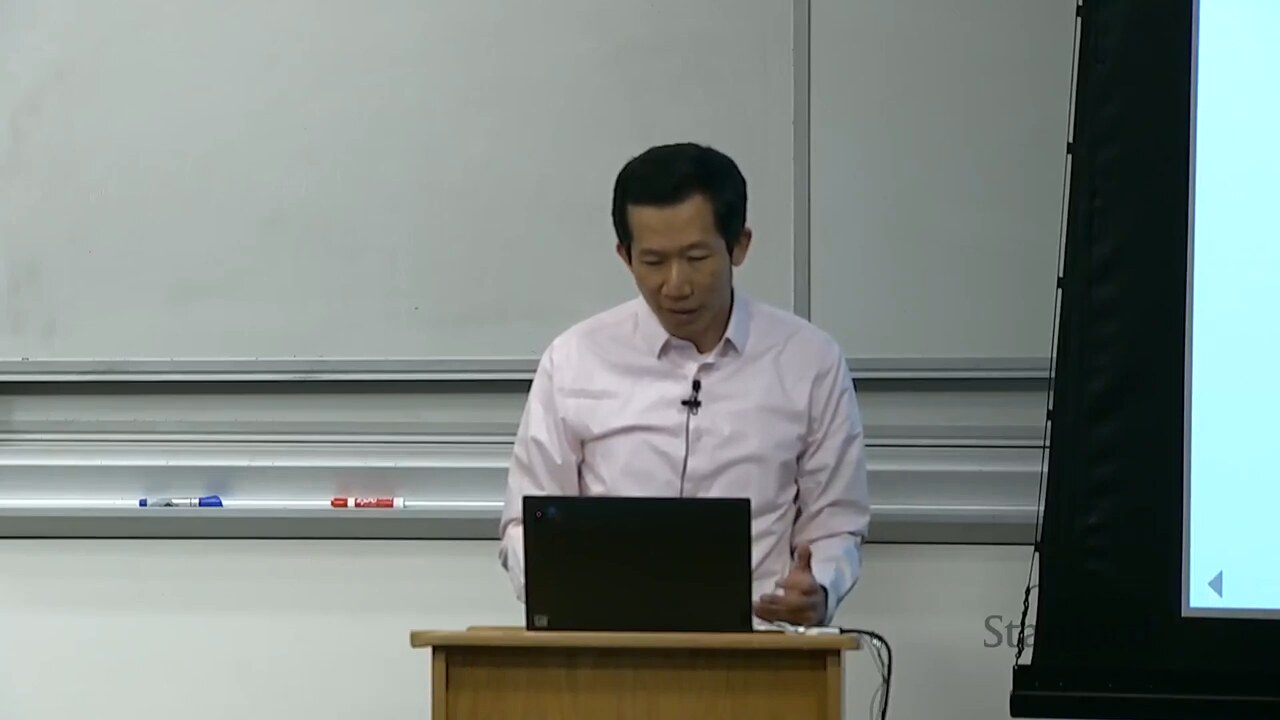
\includegraphics[width=\textwidth]{figures/fig_01_collectives_overview.jpg}
\caption{三种并行维度的全景：沿 batch / 宽度（hidden dim）/ 深度（layers）切分\protect\footnotemark}
\end{figure}
\footnotetext{视频画面时间区间：00:01:15--00:01:45。}

\begin{tabular}{p{2.5cm}p{3cm}p{8cm}}
\toprule
\textbf{并行方式} & \textbf{切分维度} & \textbf{每张卡拿到什么} \\
\midrule
数据并行（DP） & batch 维 & 完整模型 + 一份不同的数据子集 \\
张量并行（TP） & 宽度（hidden dim） & 完整数据 + 每层参数的一块切片 \\
流水线并行（PP） & 深度（layers） & 完整数据 + 连续的若干层 \\
\bottomrule
\end{tabular}

\begin{warningbox}{本讲的教学策略}
Percy 用一个\textbf{最朴素的 4 层 MLP}来演示三种并行。理由是：在当前规模下，MLP 的矩阵乘是 compute bottleneck（而非 attention），所以 MLP 足以代表真实训练的核心计算模式，又能把并行的机制看得一清二楚。但真要用在 Transformer 上时，代码复杂度会暴涨（见第 \ref{sec:3d} 节）。
\end{warningbox}

\section{集合通信原语：并行的字母表}

\subsection{术语：world size 与 rank}

在进入具体原语前，先固定术语：

\begin{importantbox}{两个核心术语}
\begin{itemize}
\item \textbf{world size}：参与这次集合通信的设备总数（如 4 块 GPU）。
\item \textbf{rank}：某台设备的编号（rank 0, rank 1, ..., rank $N{-}1$）。\emph{注意：这里的 rank 与线性代数里的"秩"无关，只是一个设备 ID。}
\end{itemize}
\end{importantbox}

\subsection{七个原语的总览}

集合通信（collective communication）是多 GPU 并行的"字母表"。下面七个原语经久耐用，几乎所有并行策略都由它们组合而成：

\begin{figure}[H]
\centering
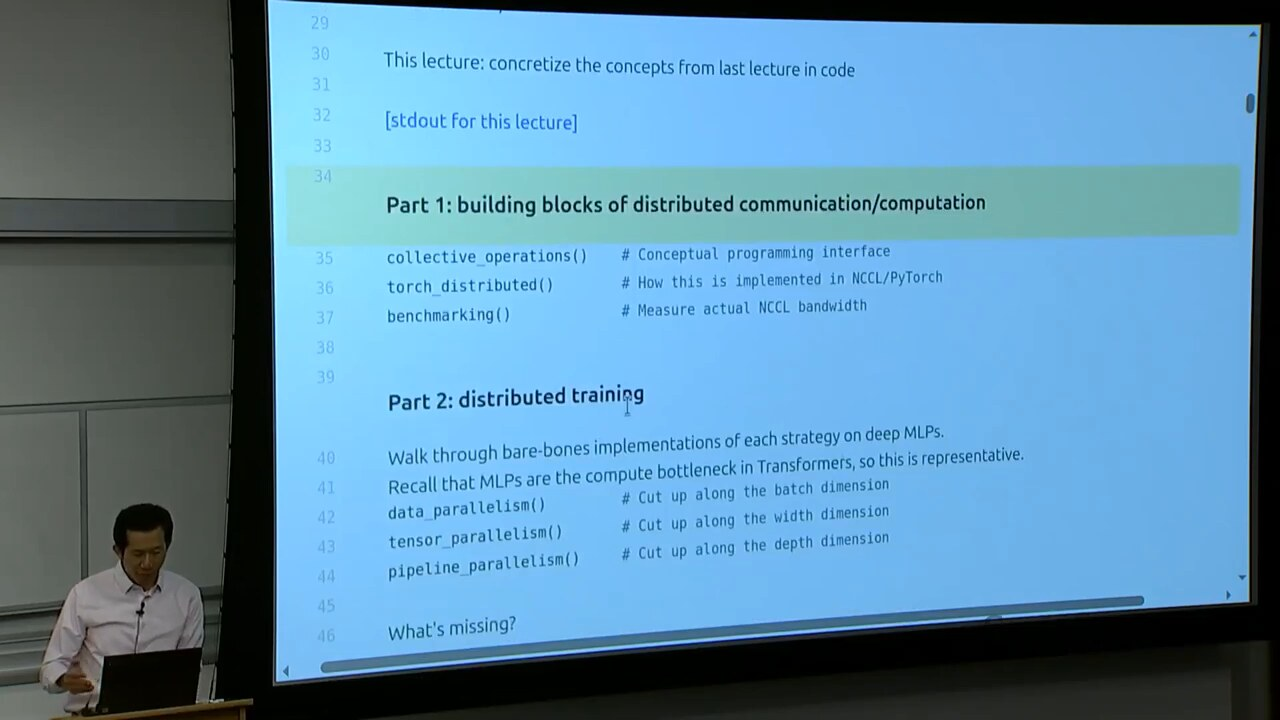
\includegraphics[width=\textwidth]{figures/fig_02_collective_ops.jpg}
\caption{七个集合通信原语总览：broadcast / scatter / gather / reduce / all-reduce / reduce-scatter / all-gather\protect\footnotemark}
\end{figure}
\footnotetext{视频画面时间区间：00:04:15--00:04:45。}

\begin{figure}[H]
\centering
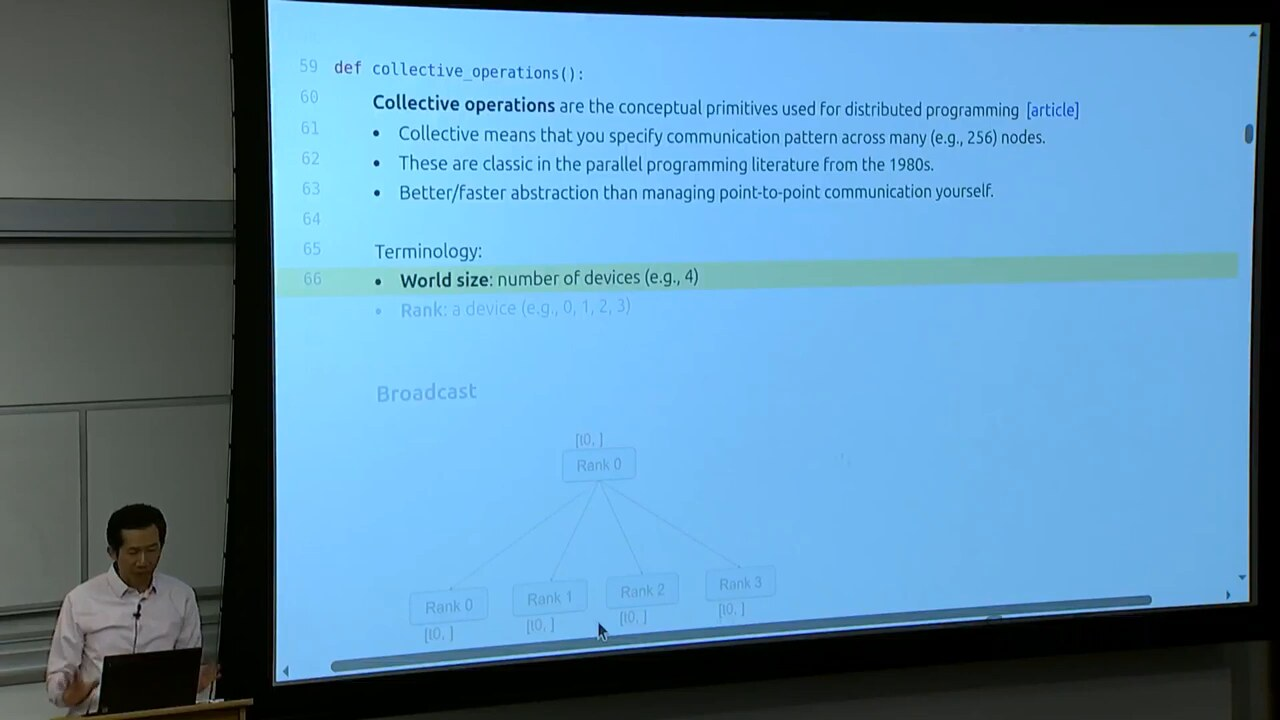
\includegraphics[width=\textwidth]{figures/fig_03_broadcast_scatter.jpg}
\caption{broadcast（同一值发全员）vs scatter（不同值分发到各 rank）\protect\footnotemark}
\end{figure}
\footnotetext{视频画面时间区间：00:05:00--00:05:30。}

\begin{tabular}{p{2.5cm}p{4.5cm}p{6.5cm}}
\toprule
\textbf{原语} & \textbf{行为} & \textbf{说明} \\
\midrule
broadcast & 一个 rank 的张量复制到所有 rank & $t_0 \to$ 全员 \\
scatter & 一个 rank 的多块张量分发到不同 rank & 每个 rank 拿到\textbf{不同}的一块 \\
gather & 各 rank 的张量拼接到一个 rank & scatter 的逆，拼接（concat） \\
reduce & 各 rank 的张量按算子合并到一个 rank & 类似 gather，但用 sum/min/max 而非拼接 \\
all-reduce & reduce 到\textbf{所有} rank & = reduce-scatter + all-gather \\
reduce-scatter & reduce 后把结果\textbf{分块}到各 rank & 每个 rank 拿到合并结果的一块 \\
all-gather & 各 rank 的张量拼接到\textbf{所有} rank & gather 的"all"版本 \\
\bottomrule
\end{tabular}

\begin{figure}[H]
\centering
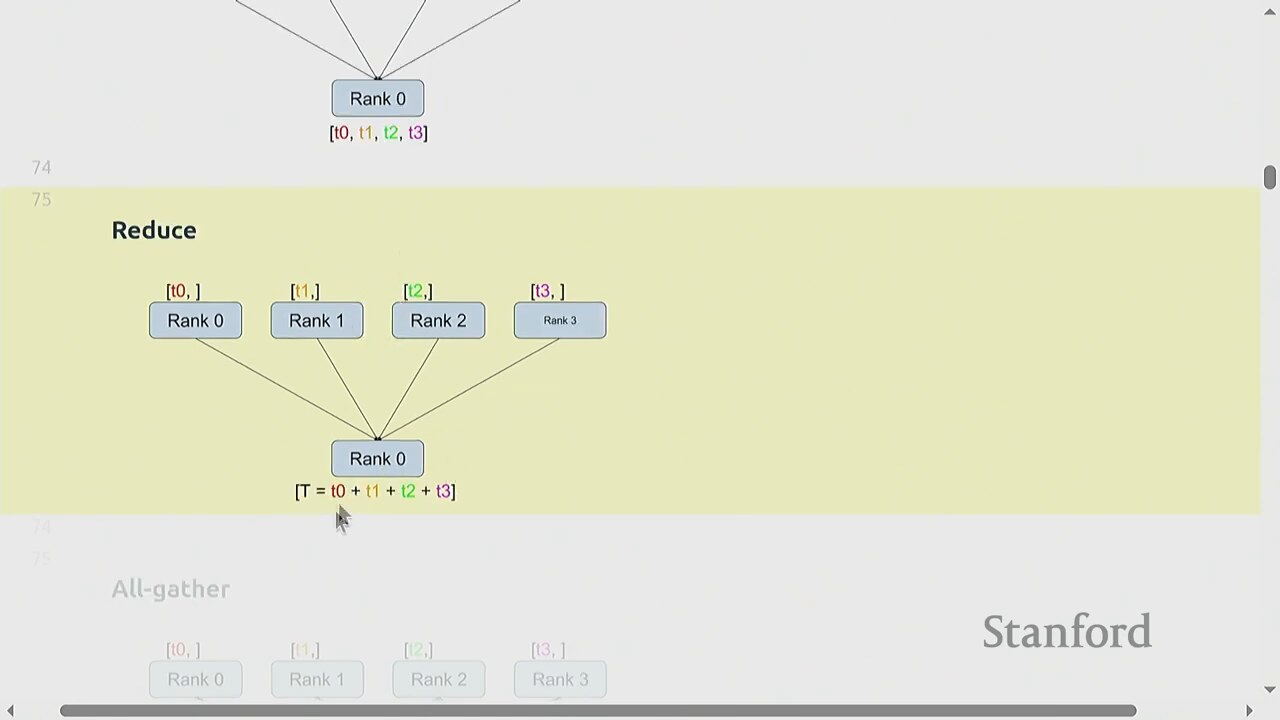
\includegraphics[width=\textwidth]{figures/fig_04_gather_reduce.jpg}
\caption{gather（拼接）vs reduce（用 sum 等算子合并到一个 rank）\protect\footnotemark}
\end{figure}
\footnotetext{视频画面时间区间：00:06:00--00:06:30。}

\begin{figure}[H]
\centering
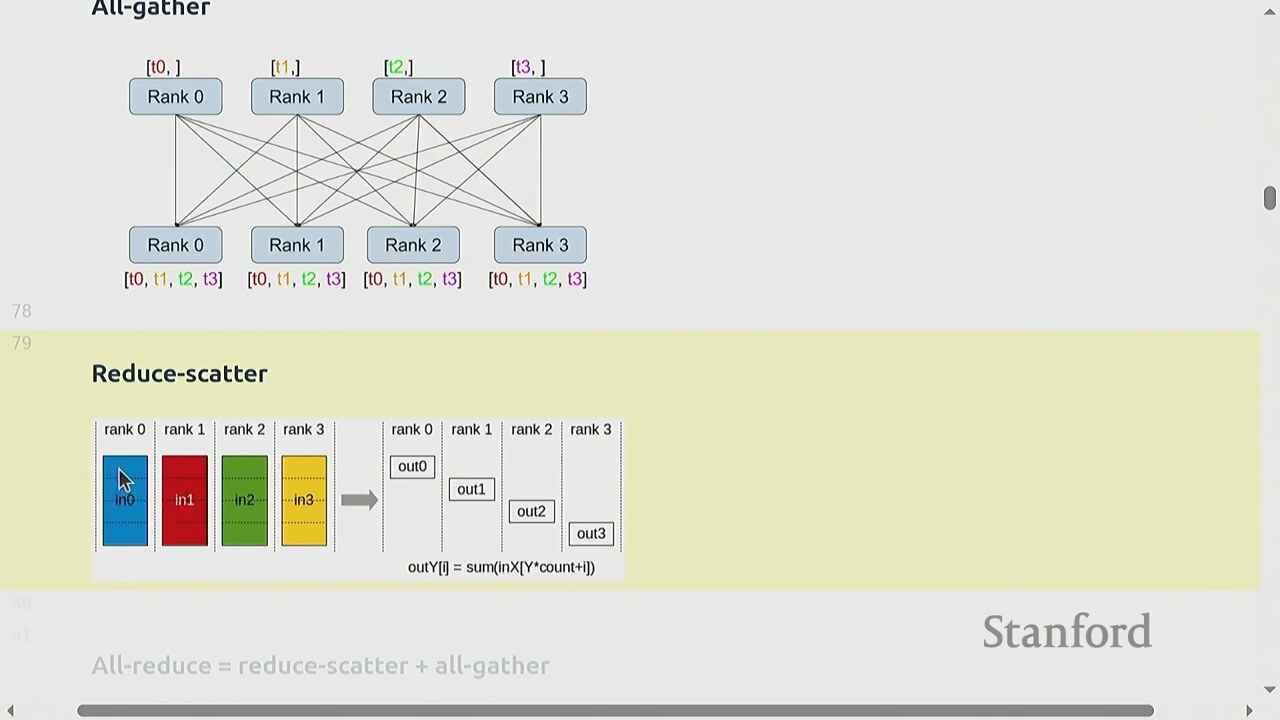
\includegraphics[width=\textwidth]{figures/fig_05_reduce_scatter.jpg}
\caption{reduce-scatter：先 reduce 再 scatter，每个 rank 拿到合并结果的一块\protect\footnotemark}
\end{figure}
\footnotetext{视频画面时间区间：00:06:30--00:07:00。}

\begin{figure}[H]
\centering
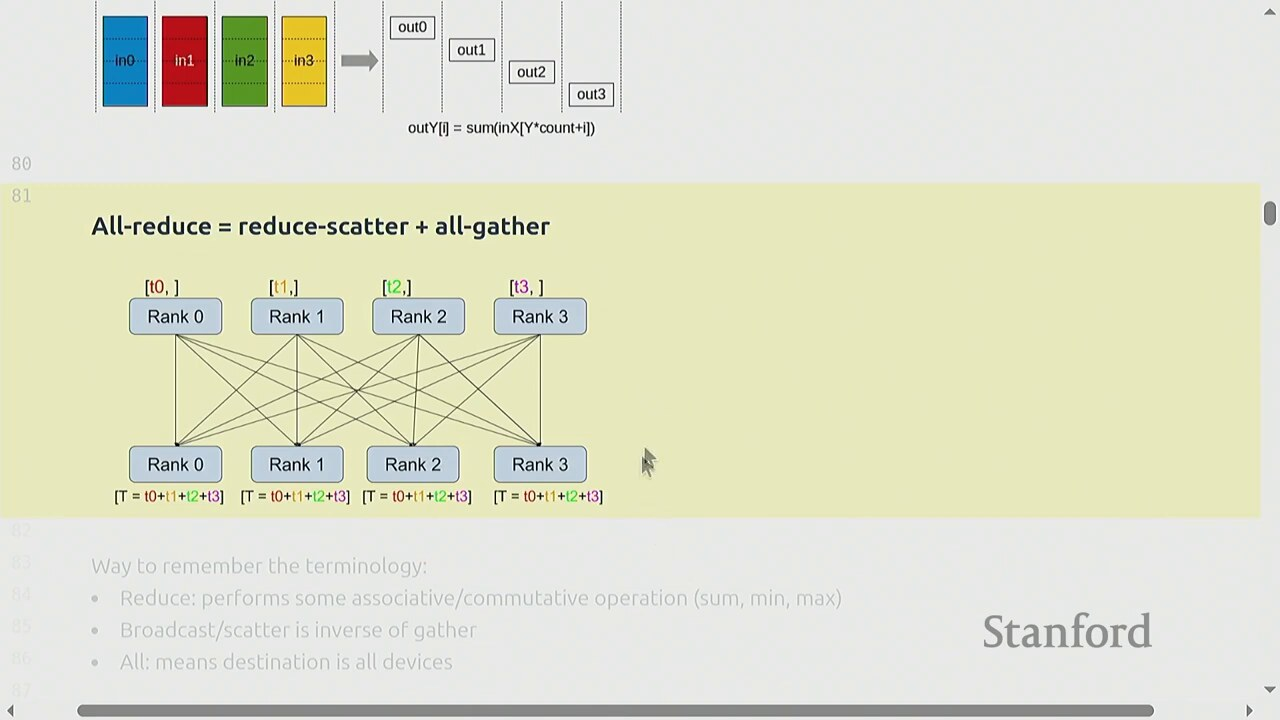
\includegraphics[width=\textwidth]{figures/fig_06_all_gather.jpg}
\caption{all-gather：各 rank 的分块拼接后，所有 rank 都拿到完整张量\protect\footnotemark}
\end{figure}
\footnotetext{视频画面时间区间：00:07:00--00:07:30。}

\subsection{最关键的一组等价关系}

\begin{figure}[H]
\centering
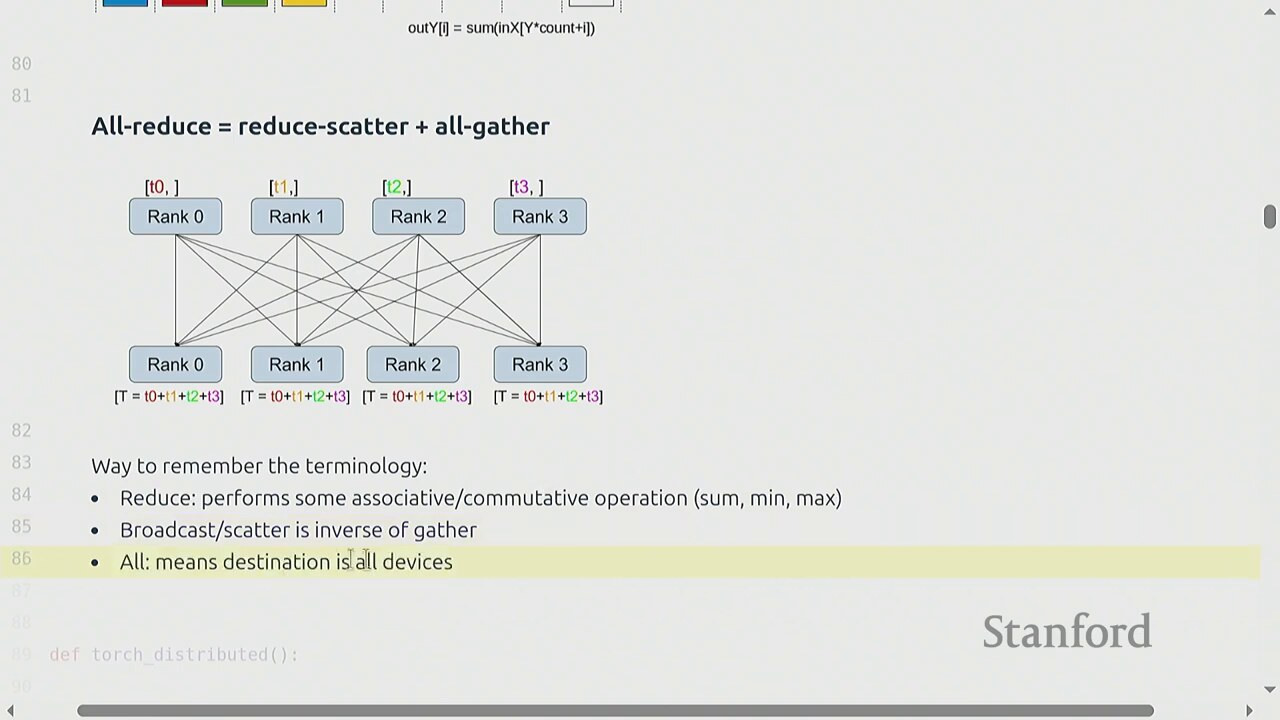
\includegraphics[width=\textwidth]{figures/fig_07_reduce_gather_inverse.jpg}
\caption{原语之间的关系：reduce = reduce-scatter + all-gather；broadcast/scatter 与 gather 互逆\protect\footnotemark}
\end{figure}
\footnotetext{视频画面时间区间：00:07:30--00:08:00。}

记忆这套术语的关键，是一组分解关系。设 $N$ 为 world size，张量 $T$ 被均分为 $N$ 块 $T_0,\dots,T_{N-1}$：

\begin{knowledgebox}{记忆口诀}
\begin{itemize}
\item \textbf{reduce} = 做\textbf{结合律/交换律}运算（sum / min / max / mean）。
\item \textbf{scatter / broadcast} 是 \textbf{gather} 的逆。
\item \textbf{all} = 目的地是\textbf{所有}设备。
\end{itemize}
\end{knowledgebox}

最核心的恒等式是：

\[
\text{all-reduce} \;=\; \text{reduce-scatter} \;+\; \text{all-gather}
\]

\begin{itemize}
\item reduce-scatter：各 rank 把按位求和的结果\textbf{分块}，每个 rank 持有总和的一块。
\item all-gather：把这一块\textbf{拼回}完整张量，于是每个 rank 都拿到完整总和。
\end{itemize}

这个恒等式不仅是记忆工具，更是后面分析通信成本和 ZeRO/FSDP 设计的基石。

\subsection{PyTorch 中的 API}

在 PyTorch 分布式（\texttt{torch.distributed}）里，这些原语都是现成的调用：

\begin{figure}[H]
\centering
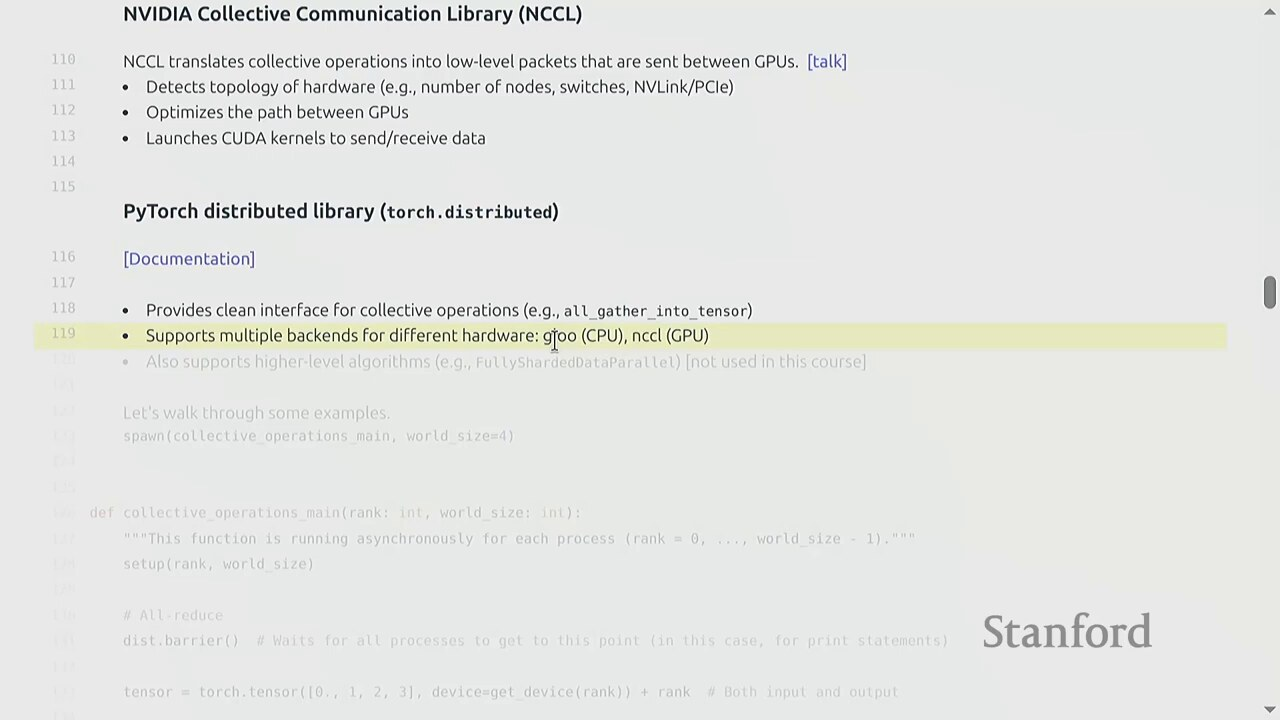
\includegraphics[width=\textwidth]{figures/fig_08_pytorch_distributed.jpg}
\caption{PyTorch 分布式 API：dist.all\_reduce / all\_gather / reduce\_scatter 的用法\protect\footnotemark}
\end{figure}
\footnotetext{视频画面时间区间：00:15:15--00:15:45。}

\begin{lstlisting}[language=Python]
import torch.distributed as dist
# all-reduce: 所有 rank 的梯度求平均后，全员持有相同结果
dist.all_reduce(param.grad, op=dist.ReduceOp.SUM)
# reduce-scatter: 输入分块求和，输出分散到各 rank
dist.reduce_scatter(output_list, input_list)
# all-gather: 各 rank 的分块拼接到所有 rank
dist.all_gather(output_list, local_tensor)
\end{lstlisting}

\section{用数值演示验证等价关系}

Percy 用一个具体的数值例子，让听众"亲眼"看到 reduce-scatter + all-gather 确实等于 all-reduce。设 world size = 4，每个 rank 持有一个含 4 个元素的张量。

\begin{figure}[H]
\centering
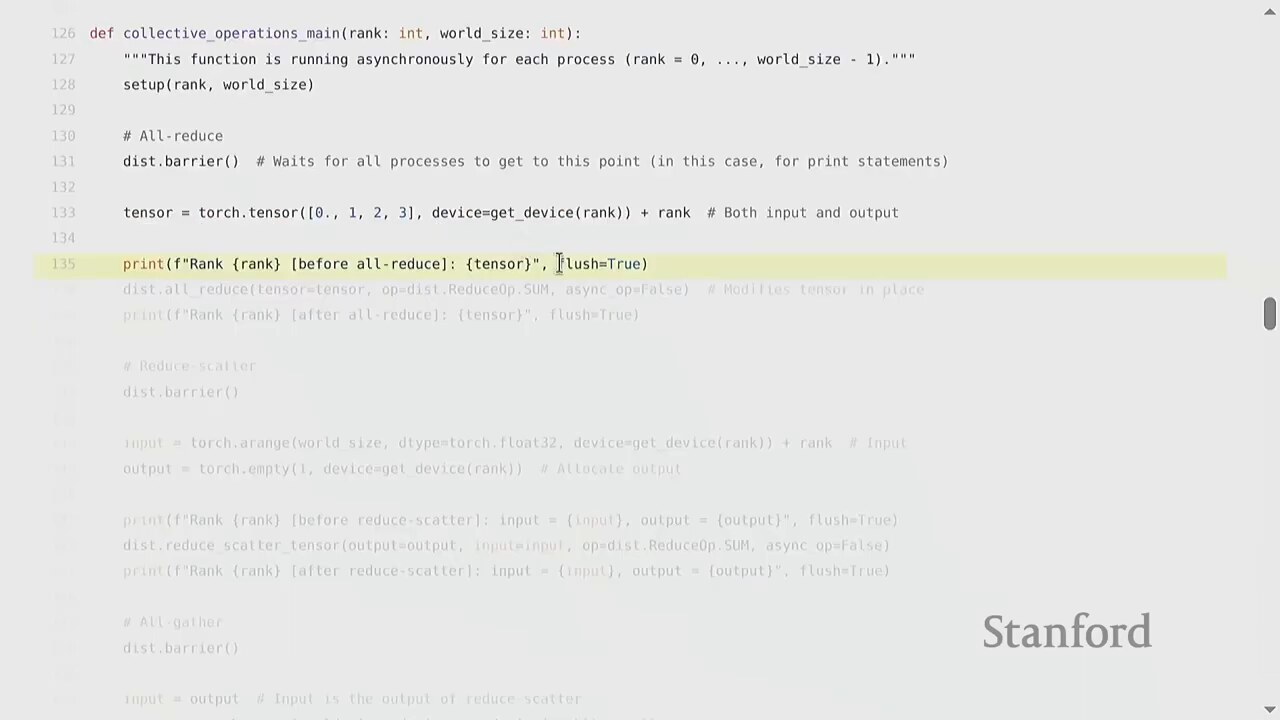
\includegraphics[width=\textwidth]{figures/fig_09_reduce_scatter_demo.jpg}
\caption{reduce-scatter 数值演示：4 个 rank 各持 $[0,1,2,3]$ 类的块，求和后各拿一列\protect\footnotemark}
\end{figure}
\footnotetext{视频画面时间区间：00:18:45--00:19:15。}

\textbf{第一步：reduce-scatter}。每个 rank 的张量被分成 4 列，按列求和：

\[
\text{rank } r \text{ 拿到第 } r \text{ 列之和} \quad\Rightarrow\quad \text{rank}_0 \to 6,\; \text{rank}_1 \to 10,\; \text{rank}_2 \to 14,\; \text{rank}_3 \to 18
\]

\textbf{第二步：all-gather}。把这 4 个结果拼回：

\begin{figure}[H]
\centering
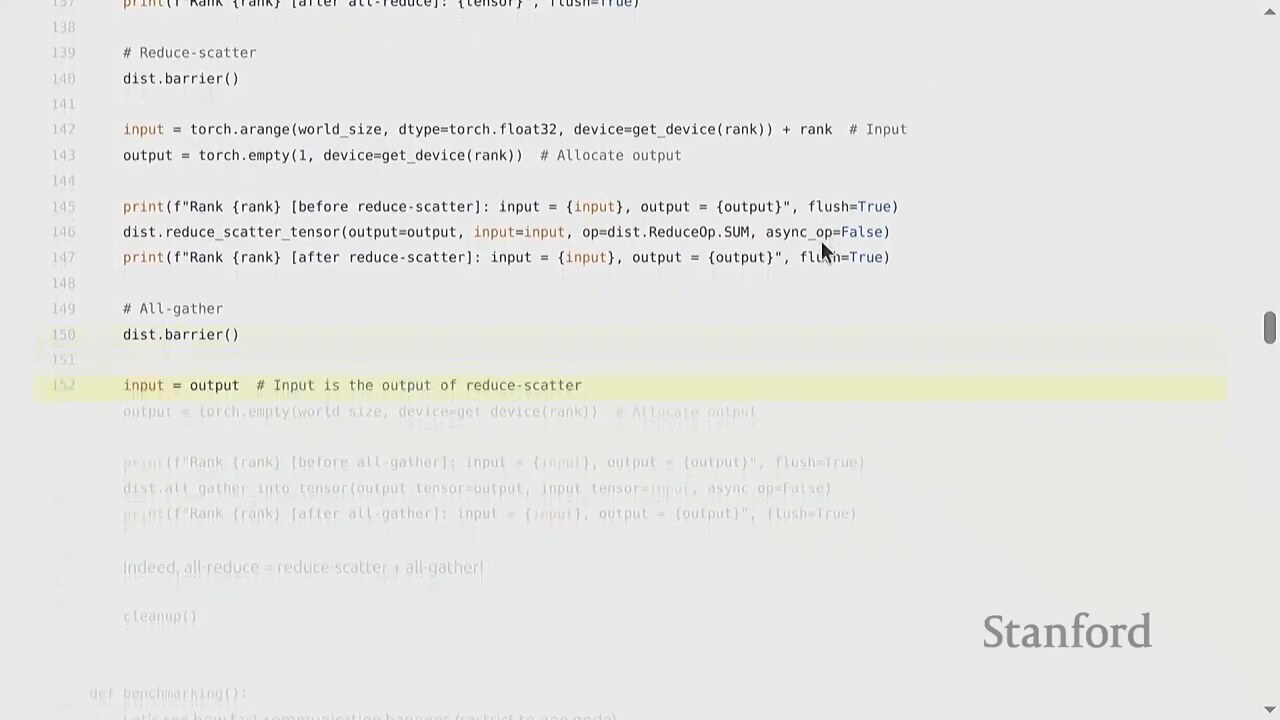
\includegraphics[width=\textwidth]{figures/fig_10_all_gather_demo.jpg}
\caption{all-gather 演示：把 reduce-scatter 的分块输出拼回 $[6,10,14,18]$，与 all-reduce 结果一致\protect\footnotemark}
\end{figure}
\footnotetext{视频画面时间区间：00:21:00--00:21:30。}

\[
\text{所有 rank 最终都拿到 } [6,\,10,\,14,\,18]
\]

\begin{practicebox}{演示的结论}
reduce-scatter + all-gather 产出的结果，和直接做一次 all-reduce \textbf{逐位相等}。这验证了恒等式 $\text{all-reduce} = \text{reduce-scatter} + \text{all-gather}$，也为下一节分析通信成本提供了分解视角。
\end{practicebox}

\section{通信成本与带宽基准测试}

\subsection{ring all-reduce 的实现}

\begin{figure}[H]
\centering
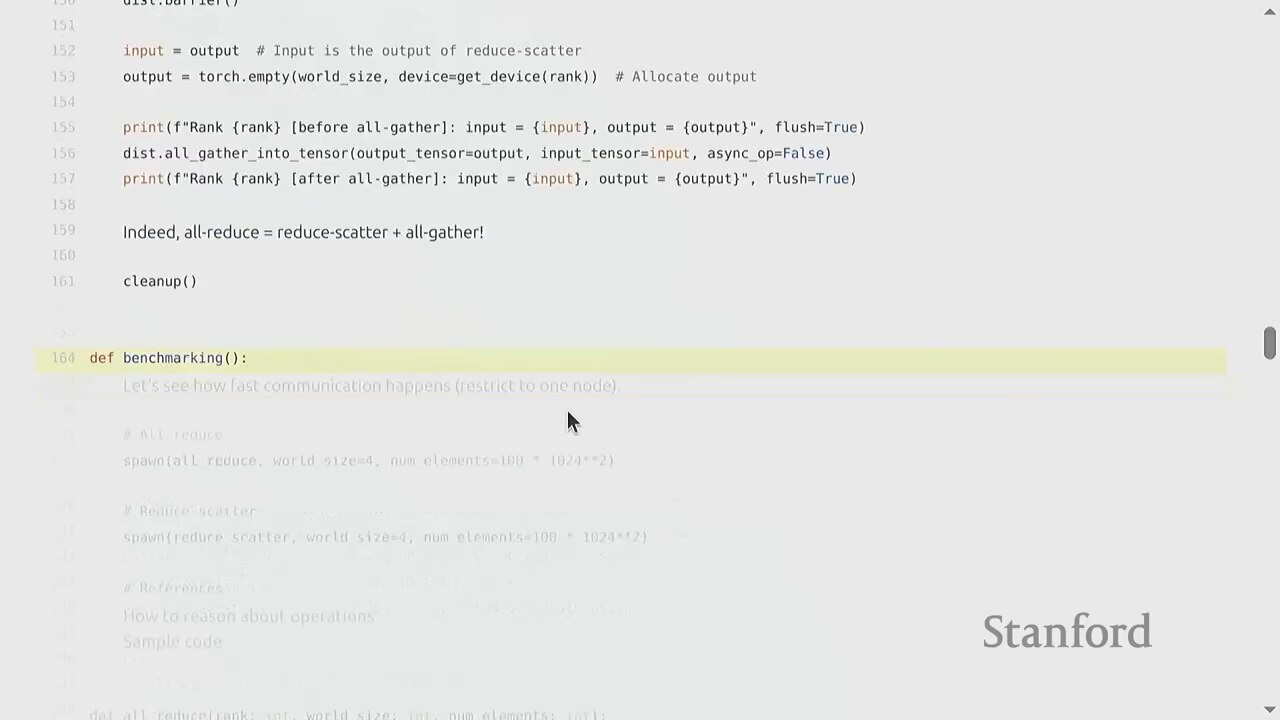
\includegraphics[width=\textwidth]{figures/fig_11_all_reduce_ring.jpg}
\caption{all-reduce 的 ring 实现：分步 reduce 再分步 broadcast，通信量为 $\frac{2(N-1)}{N}\cdot\text{size}$\protect\footnotemark}
\end{figure}
\footnotetext{视频画面时间区间：00:23:45--00:24:15。}

实际的 all-reduce 通常用 \textbf{ring} 拓扑实现：把 $N$ 个 rank 排成环，数据沿环分两阶段流动——先 reduce（每步每个 rank 收一块、合并、再传下一站），再 broadcast（逆向把完整结果传遍全环）。

设张量大小为 $S$ 字节，world size 为 $N$，则每个 rank 在整个 ring all-reduce 中实际\textbf{发出}的数据量为：

\[
\text{每 rank 发送量} = \frac{2(N-1)}{N} \cdot S
\]

\begin{itemize}
\item 系数 2：来自两个阶段（reduce-scatter 阶段 + all-gather 阶段），各贡献 $\frac{N-1}{N}S$。
\item 当 $N$ 很大时，$\frac{2(N-1)}{N} \to 2$，即每 rank 接近发送 $2S$ 字节。
\end{itemize}

\subsection{如何测量带宽}

\begin{figure}[H]
\centering
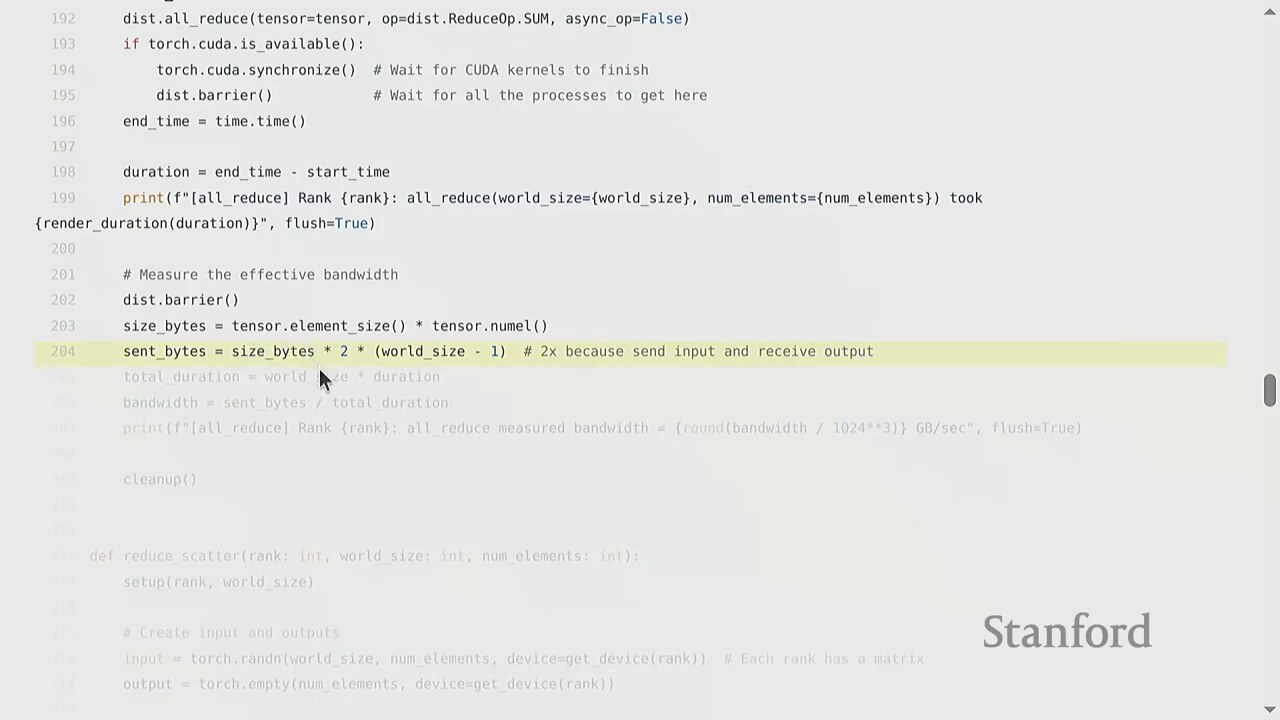
\includegraphics[width=\textwidth]{figures/fig_12_bandwidth_benchmark.jpg}
\caption{带宽基准测试：测量 all-reduce 在不同张量大小下的耗时与字节传输量\protect\footnotemark}
\end{figure}
\footnotetext{视频画面时间区间：00:26:15--00:26:45。}

基准测试有严格的"清口"流程，避免把 kernel 加载、warmup 的开销算进计时：

\begin{enumerate}
\item \textbf{warm up}：先跑一次操作，再 \texttt{synchronize + barrier}，确保所有 kernel 已加载、缓存已就位。
\item \textbf{start clock}：记录起始时间。
\item 执行 \texttt{all\_reduce}。
\item \textbf{sync + stop clock}：同步后停止计时。
\item 用"实际传输字节数 / 耗时"得到聚合带宽。
\end{enumerate}

\begin{warningbox}{基准测试的陷阱}
GPU kernel 是\textbf{异步}下发的——你调用 \texttt{all\_reduce} 立刻返回，但计算可能还在排队。所以\textbf{必须}在 stop clock 前做 \texttt{torch.cuda.synchronize()}，否则你测的是"下发时间"而非"执行时间"。warmup 也是同理：第一次调用要把 kernel 编译/加载进缓存，这一步极慢，不能计入。
\end{warningbox}

传输字节数的计算：张量有 $\text{numel}$ 个元素，每个元素 \texttt{float32} 占 4 字节，故张量字节数为：

\[
\text{size} = \text{numel} \times \text{element\_bytes} = \text{numel} \times 4
\]

聚合带宽（aggregate bandwidth，单位 GB/s）为：

\[
B = \frac{\text{size} \times \frac{2(N-1)}{N}}{T_{\text{elapsed}}}
\]

\subsection{为什么 all-reduce 有 2x 因子}

这是本节最微妙、也是被反复追问的一点。

\begin{figure}[H]
\centering
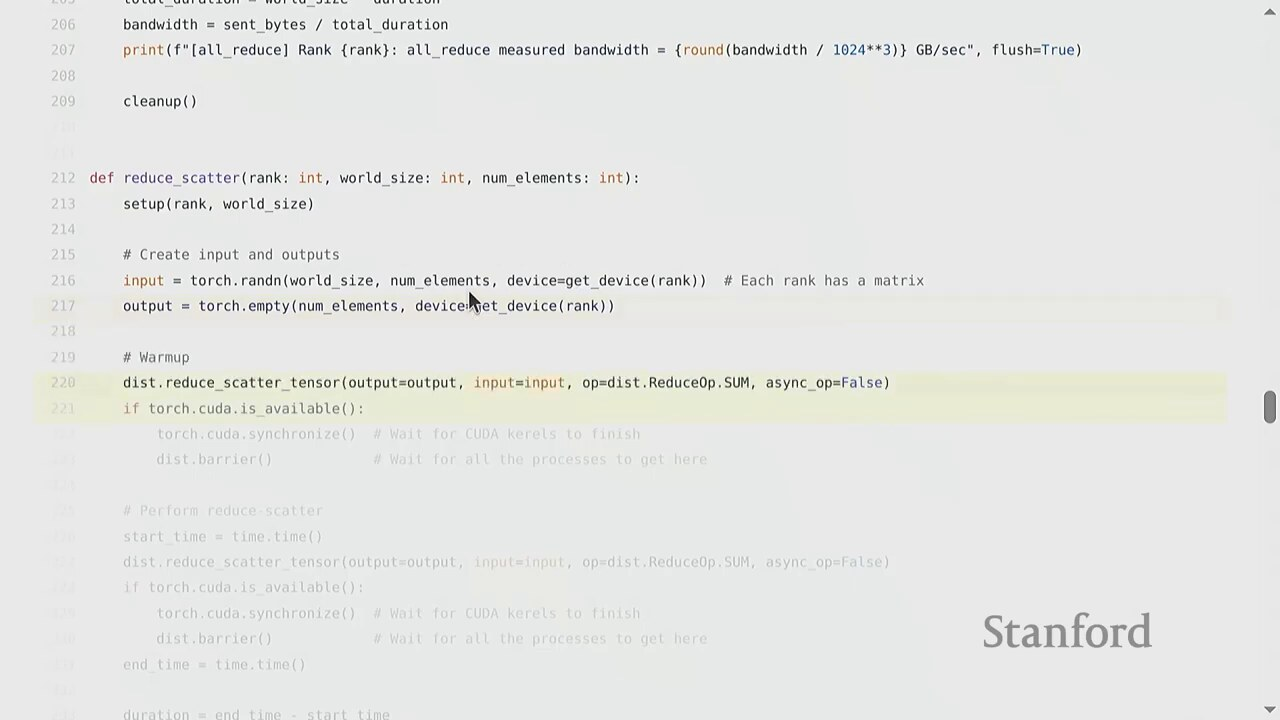
\includegraphics[width=\textwidth]{figures/fig_13_reduce_scatter_bench.jpg}
\caption{reduce-scatter 基准测试：与 all-reduce 对比，\textbf{没有} 2x 因子\protect\footnotemark}
\end{figure}
\footnotetext{视频画面时间区间：00:28:30--00:29:00。}

\begin{importantbox}{2x 因子的来源}
\begin{itemize}
\item \textbf{all-reduce = reduce-scatter + all-gather}，两步各传输 $\frac{N-1}{N}S$，加起来 $\frac{2(N-1)}{N}S$ —— 这是 "2x"。
\item \textbf{reduce-scatter 单独}只做一步，传输量是 $\frac{N-1}{N}S$，\textbf{没有} 2x。
\item \textbf{all-gather 单独}也只有 $\frac{N-1}{N}S$，\textbf{没有} 2x。
\end{itemize}
\end{importantbox}

课堂上的追问澄清了一个易混点：reduce-scatter 名字里虽含 "reduce"，但 NCCL 底层可能用硬件加速把 reduce 和 scatter 融合，实际只算一次传输。Percy 强调：\textbf{"它叫 reduce-scatter，但其实就是一次 reduction"}。于是从字节计数的角度：

\[
\text{all-reduce 传输量} = \underbrace{\text{reduce-scatter 传输量}}_{\frac{N-1}{N}S} + \underbrace{\text{all-gather 传输量}}_{\frac{N-1}{N}S} = \frac{2(N-1)}{N}S
\]

\begin{figure}[H]
\centering
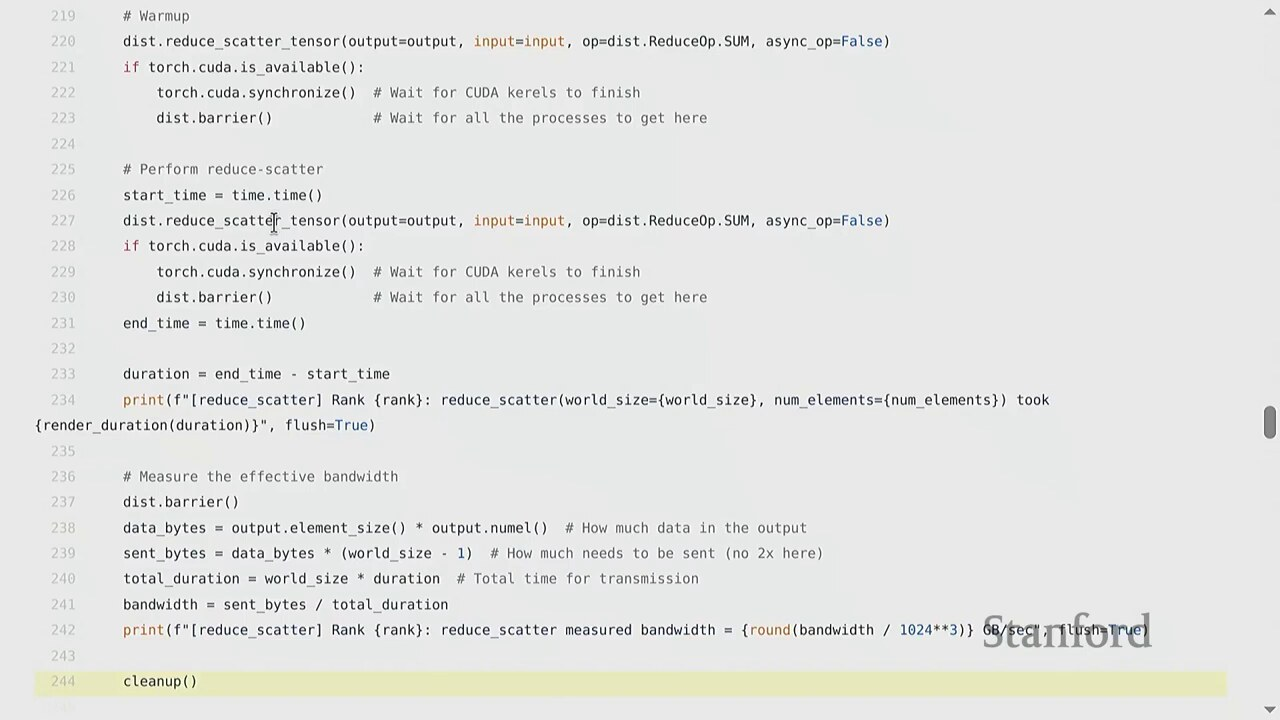
\includegraphics[width=\textwidth]{figures/fig_14_comm_cost_analysis.jpg}
\caption{通信成本分析：reduce-scatter 与 all-gather 各 $\frac{N-1}{N}S$，all-reduce 是二者之和\protect\footnotemark}
\end{figure}
\footnotetext{视频画面时间区间：00:31:15--00:31:45。}

\begin{knowledgebox}{为什么要费这么大劲算字节？}
因为\textbf{带宽是通信瓶颈的硬约束}。知道一次集合通信要搬多少字节、硬件能跑多快，你就能在写代码前\textbf{预测}它会不会成为瓶颈——而不是等训练跑起来才发现卡在通信上。这是 systems 心态的核心：先算账，再动手。
\end{knowledgebox}

\section{数据并行（Data Parallelism / DDP）}

\subsection{沿 batch 维切分}

数据并行是最直观的并行：模型副本完整地放在每张卡上，把\textbf{数据按 batch 维切}成 $N$ 份，每张卡处理一份。

\begin{figure}[H]
\centering
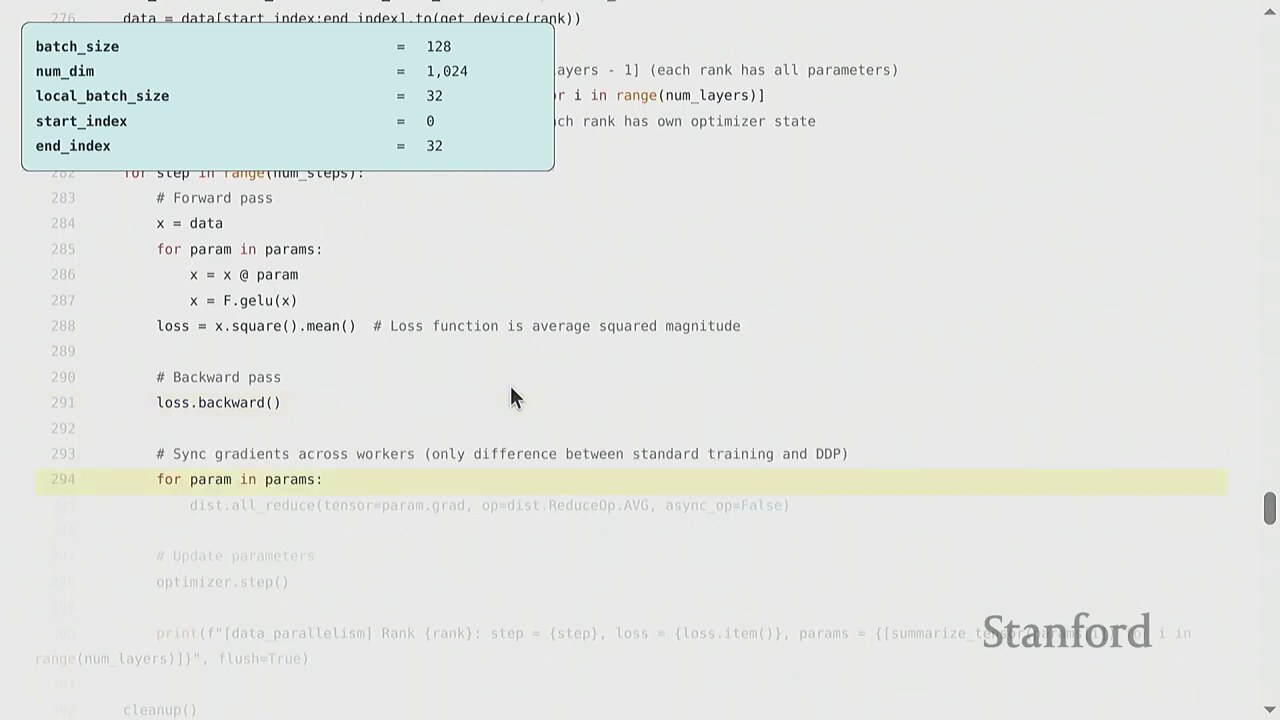
\includegraphics[width=\textwidth]{figures/fig_15_allreduce_data_parallel.jpg}
\caption{数据并行：all-reduce 的教科书应用——梯度同步\protect\footnotemark}
\end{figure}
\footnotetext{视频画面时间区间：00:36:15--00:36:45。}

设 batch size 为 $B$，hidden dim 为 $D$，world size 为 $N$。每张卡的\textbf{本地 batch} 为：

\[
B_{\text{local}} = \frac{B}{N}
\]

每个 rank 根据 rank id 取 batch 中对应的一段：

\[
\text{rank } r \text{ 取行 } [r \cdot B_{\text{local}},\; (r+1)\cdot B_{\text{local}})
\]

\subsection{DDP 的实现：在 SGD 里"注入"一行 all-reduce}

Percy 展示了 DDP 的最朴素实现：它\textbf{几乎和普通 SGD 一模一样}，唯一的区别是在反向传播之后、参数更新之前，对每个参数的梯度做一次 all-reduce（取平均）。

\begin{lstlisting}[language=Python]
for step in range(num_steps):
    out = forward(x_local, layers)      # 前向：每卡用自己的数据子集
    loss = criterion(out)
    loss.backward()                      # 反向：得到 param.grad
    for param in model.parameters():
        dist.all_reduce(param.grad, op=dist.ReduceOp.SUM)  # 同步梯度
        param.grad /= world_size         # 求平均
    optimizer.step()                     # 更新参数（和普通 SGD 完全一样）
\end{lstlisting}

\begin{figure}[H]
\centering
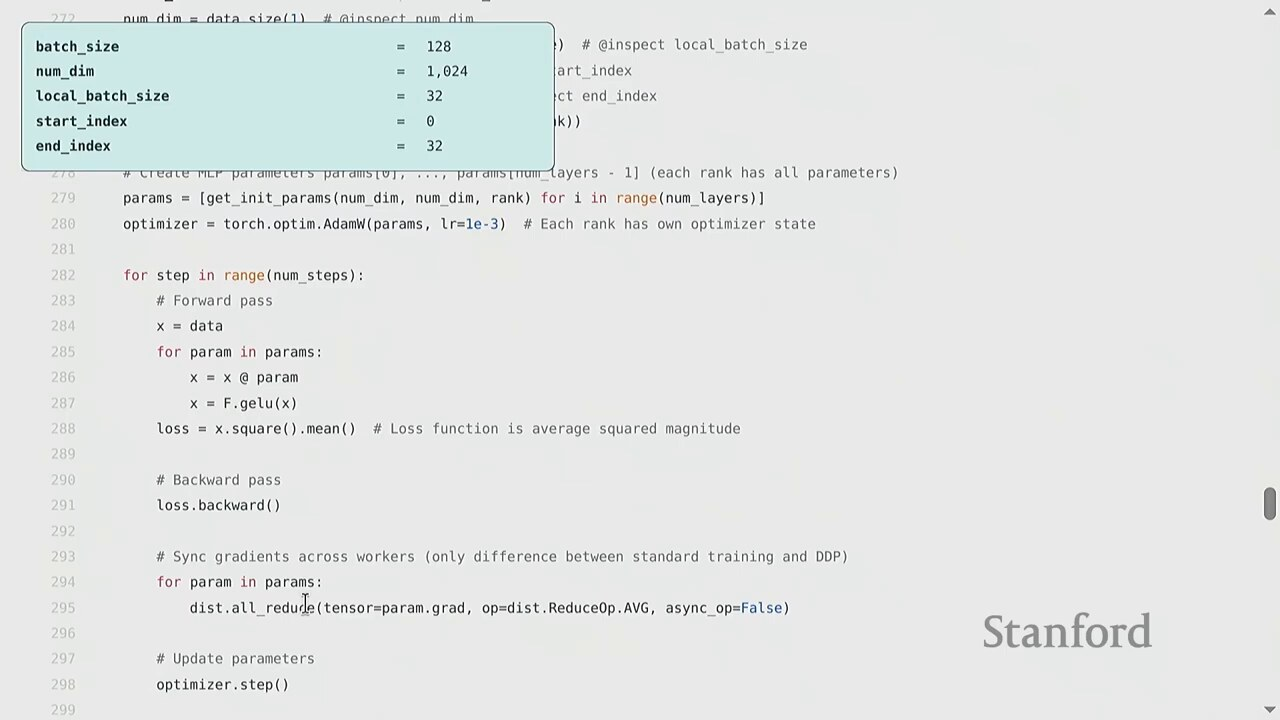
\includegraphics[width=\textwidth]{figures/fig_16_dp_gradient_sync.jpg}
\caption{数据并行梯度同步：所有 rank 在同一 step 做 all-reduce，是一个同步点\protect\footnotemark}
\end{figure}
\footnotetext{视频画面时间区间：00:38:15--00:38:45。}

\subsection{DDP 的关键性质}

\begin{importantbox}{同步语义}
\begin{itemize}
\item \textbf{loss 各卡不同}：因为每卡的数据子集不同。
\item \textbf{梯度 all-reduce 后各卡相同}：所以参数更新后各卡也相同。
\item 因此 DDP 等价于\textbf{用 $N$ 倍 batch size 跑一次同步 SGD}——只是计算被摊到了 $N$ 张卡上。
\end{itemize}
\end{importantbox}

\begin{warningbox}{all-reduce 是同步点}
all-reduce 是一个\textbf{阻塞式同步点}：所有 rank 必须都到达这一步，才能继续。如果某个 rank 漏写了一次 all-reduce（或张量形状不匹配），整个训练会\textbf{挂起（hang）}——没有任何报错，只是永远等待。这是 DDP 调试中最常见的"幽灵 bug"。课堂上有人问"如何保证各 rank 在同一 step"，答案正是：all-reduce 本身就是同步屏障。
\end{warningbox}

\begin{practicebox}{作业对应}
DDP 是 Assignment 2 的内容（在 Transformer 上实现）。本讲的 MLP 版本是它的最朴素骨架——去掉所有花哨优化，只保留"反向后 all-reduce 梯度"这一行，让机制完全透明。
\end{practicebox}

\begin{knowledgebox}{为什么不在各卡间传优化器状态？}
课堂上有一个延伸问题：既然要同步，为什么不干脆把\textbf{优化器状态}（Adam 的一阶/二阶矩）在各卡间搬运同步，而要各卡各自维护？答案在于效率：优化器状态的更新（几个逐元素运算）远比把它在网络上搬运一次要\textbf{便宜得多}。所以正确做法是：每卡各自动维护一份完整优化器状态，只在梯度上做 all-reduce。这是一种典型的"宁可多算一点，也不愿多搬一点"的权衡——计算是廉价的，搬运是昂贵的。
\end{knowledgebox}

\section{张量并行（Tensor Parallelism，Megatron 风格）}

\subsection{沿 hidden dim 切分模型}

数据并行切数据，张量并行则切\textbf{模型本身}：把每一层的参数矩阵沿 hidden 维（宽度）切成 $N$ 块，每张卡持有一块。数据则完整地在各卡间流转。

\begin{figure}[H]
\centering
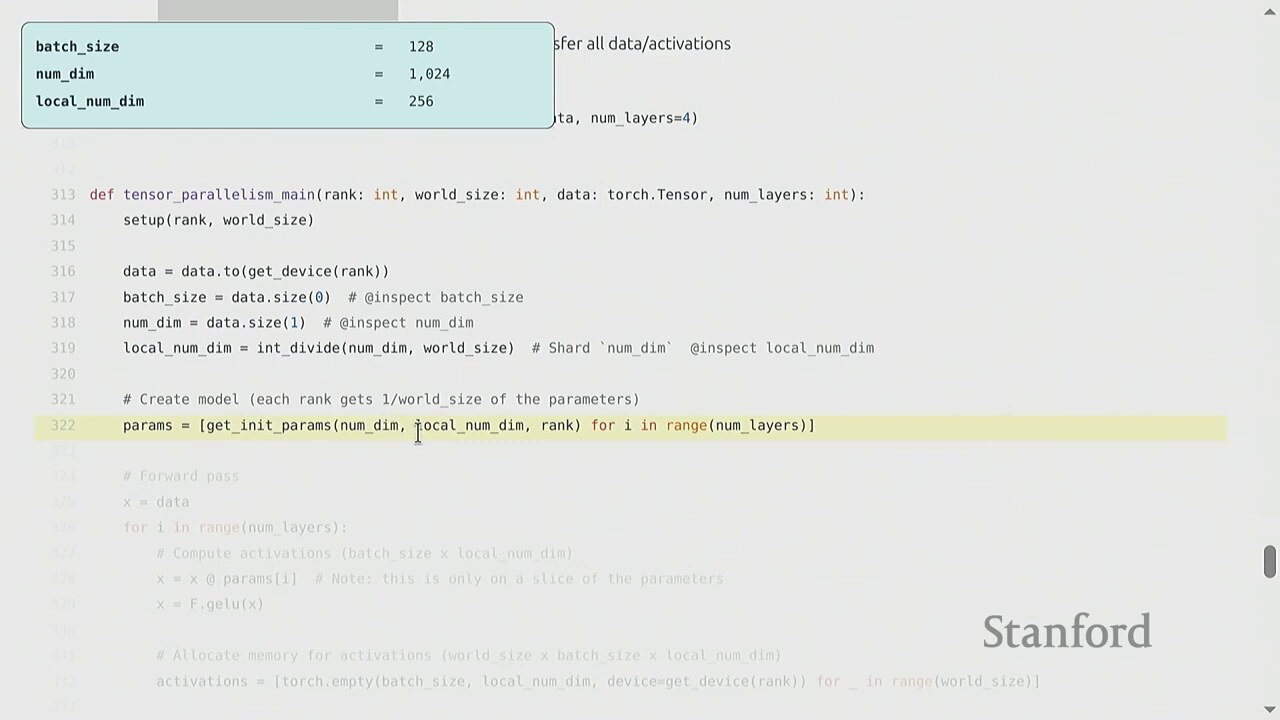
\includegraphics[width=\textwidth]{figures/fig_17_tensor_parallel_split.jpg}
\caption{张量并行：把模型沿 hidden dim 切分，local\_num\_dim = num\_dim / world\_size\protect\footnotemark}
\end{figure}
\footnotetext{视频画面时间区间：00:41:45--00:42:15。}

设 hidden dim 为 $D$，world size 为 $N$，则每卡的本地维度为：

\[
D_{\text{local}} = \frac{D}{N}
\]

例如 $D = 1024,\; N = 4$，则 $D_{\text{local}} = 256$。每张卡的参数矩阵形状从 $D \times D$ 变为 $D \times D_{\text{local}}$，即每卡只持有 $\frac{1}{N}$ 的参数。

\begin{importantbox}{为什么要切模型？}
因为\textbf{模型放不进单卡}。当模型参数量超过单卡显存时，数据并行（需要每卡存完整模型）就失效了，必须把参数本身分片。这是张量并行存在的根本理由。
\end{importantbox}

\subsection{前向传播：all-gather 拼回激活}

每张卡只持有 $\frac{1}{N}$ 的参数，所以它算出的激活也只有 $\frac{1}{N}$（形状为 $B \times D_{\text{local}}$）。要让下一层能继续算，必须把所有卡的激活\textbf{拼回}完整维度：

\begin{figure}[H]
\centering
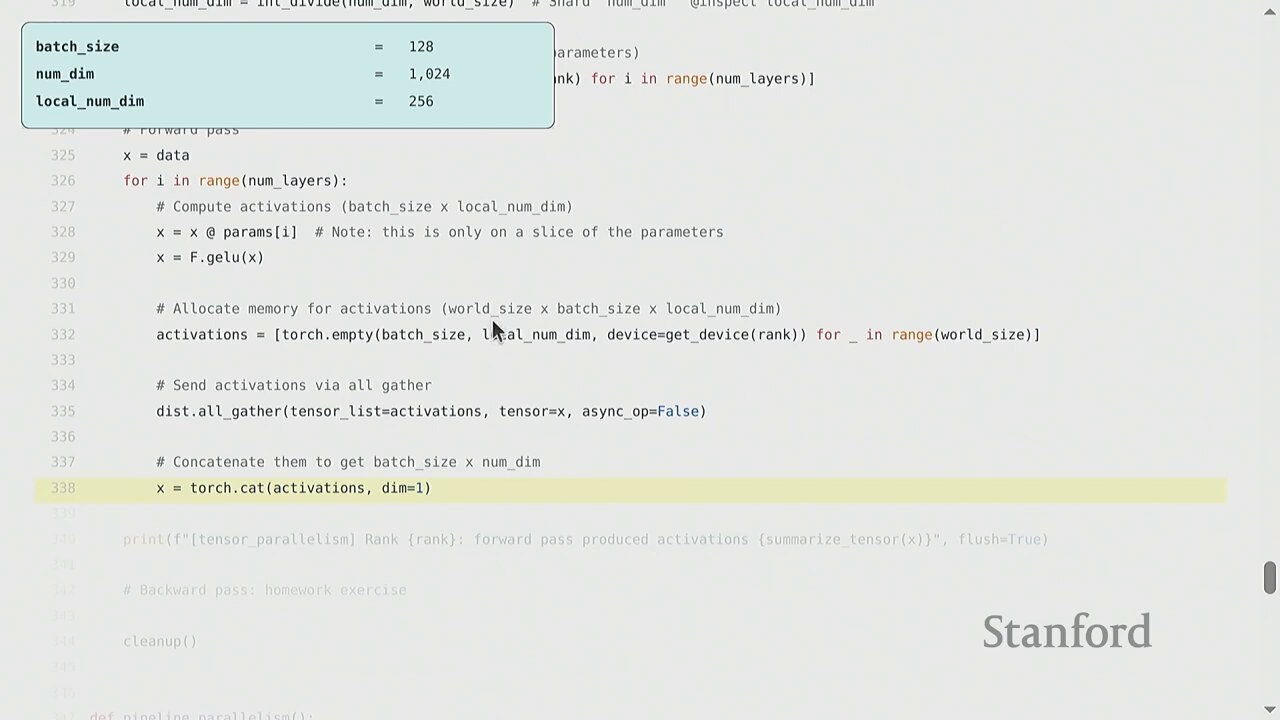
\includegraphics[width=\textwidth]{figures/fig_18_tensor_forward.jpg}
\caption{张量并行前向：每卡算自己那份，再 all-gather 拼回完整输出\protect\footnotemark}
\end{figure}
\footnotetext{视频画面时间区间：00:44:45--00:45:15。}

\begin{lstlisting}[language=Python]
for layer in layers:
    # 每卡只算 local 部分：x 形状 B x D_local
    x_local = activation(x_local, layer_local)  # 用本地参数
    # 为完整输出预留空间：world_size 份 B x D_local
    acts = [empty(B, D_local) for _ in range(world_size)]
    dist.all_gather(acts, x_local)   # 把各卡的 x_local 拼到所有卡
    x_local = cat(acts, dim=1)        # 拼接 -> B x D
\end{lstlisting}

\begin{figure}[H]
\centering
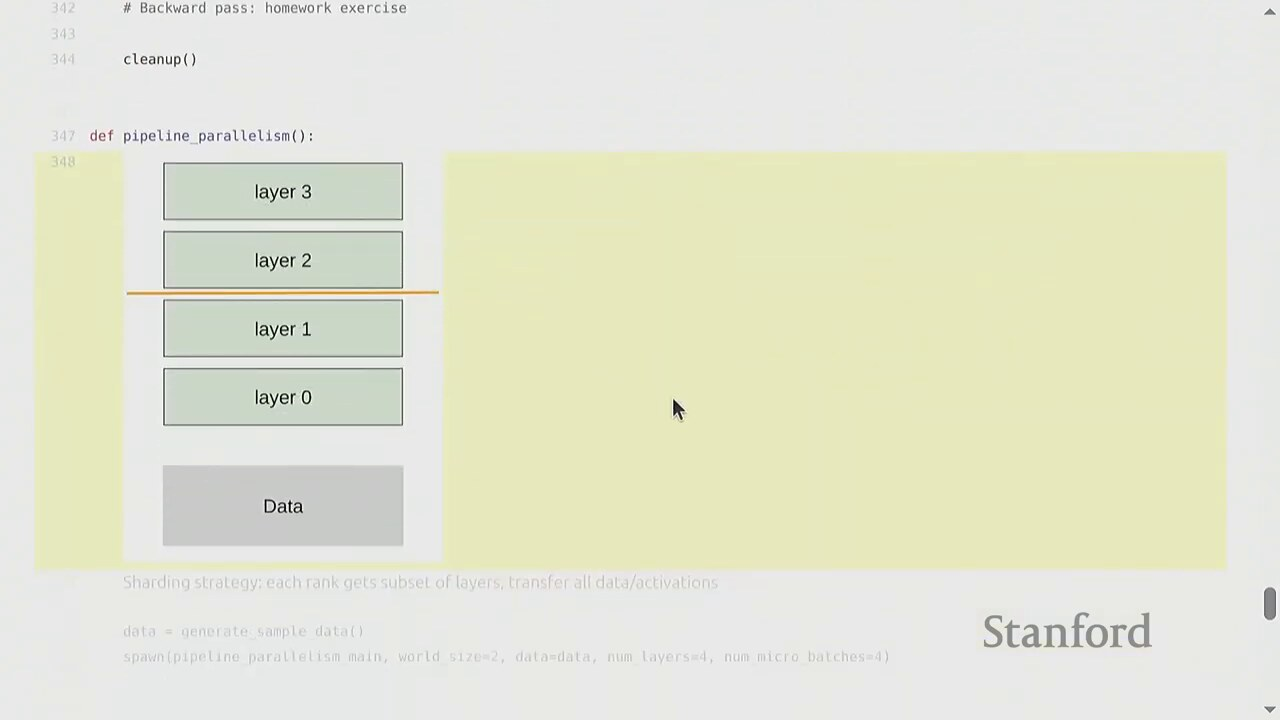
\includegraphics[width=\textwidth]{figures/fig_19_tensor_allgather.jpg}
\caption{张量并行中的 all-gather：每个 rank 持局部输出，all-gather 后全员得到完整结果\protect\footnotemark}
\end{figure}
\footnotetext{视频画面时间区间：00:46:15--00:46:45。}

\subsection{通信代价与适用场景}

\begin{warningbox}{张量并行的通信代价}
张量并行\textbf{每一层之间}都要做一次 all-gather，通信极其频繁。因此它\textbf{对互连带宽要求极高}——通常只在\textbf{节点内}（NVLink 全连接，带宽高达 900 GB/s）使用，跨节点走以太网会因通信太慢而得不偿失。
\end{warningbox}

\begin{knowledgebox}{Megatron-LM 的关键洞察}
Megatron-LM 论文指出：对 MLP 的两层结构，若把第一层按列切、第二层按行切，中间的 all-gather 可以被一次 \textbf{reduce-scatter} 替代，从而把通信量减半。这是工业级张量并行的核心优化，但本讲的朴素版只演示了最直观的 all-gather 方案。
\end{knowledgebox}

\begin{practicebox}{反向传播被略过}
Percy 在课上只演示了张量并行的\textbf{前向}，反向传播"因为时间关系略过"。反向的机制并不难（对 all-gather 求导即 reduce-scatter），但代码 bookkeeping 繁琐。完整的张量并行（含 attention 的 head 维切分、MLP 的列/行切分组合）正是 Megatron-LM 等框架的核心。
\end{practicebox}

\section{流水线并行（Pipeline Parallelism）}

\subsection{按层切分模型}

流水线并行把模型沿\textbf{深度}（layers）切：每张卡拿到\textbf{连续的若干层}，数据像流水线一样从第一张卡流向最后一张卡。

\begin{figure}[H]
\centering
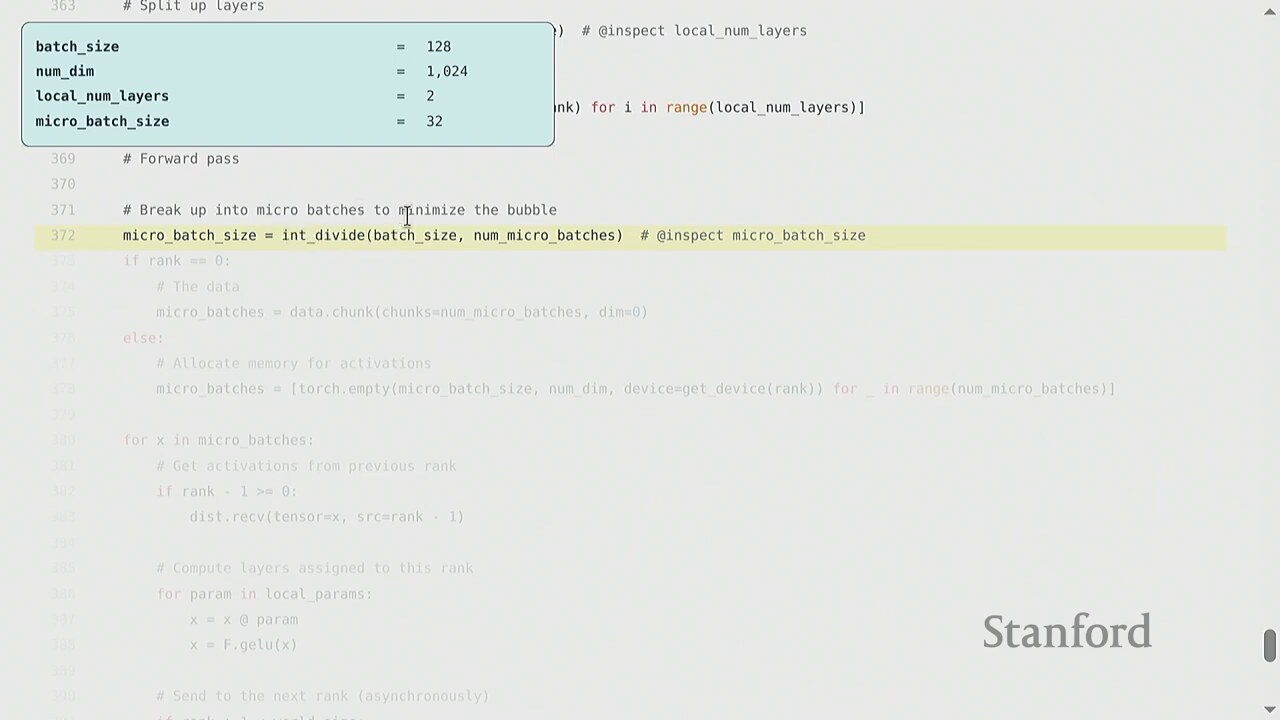
\includegraphics[width=\textwidth]{figures/fig_20_pipeline_intro.jpg}
\caption{流水线并行：把模型按层切分，相邻 stage 间用 send/recv 传递激活\protect\footnotemark}
\end{figure}
\footnotetext{视频画面时间区间：00:47:45--00:48:15。}

设模型有 $L$ 层，world size 为 $N$，则每张卡分到：

\[
L_{\text{per\_stage}} = \frac{L}{N}
\]

例如 $L = 4,\; N = 2$，则 rank 0 持第 0--1 层，rank 1 持第 2--3 层。

\subsection{气泡（bubbles）：朴素实现的代价}

\begin{figure}[H]
\centering
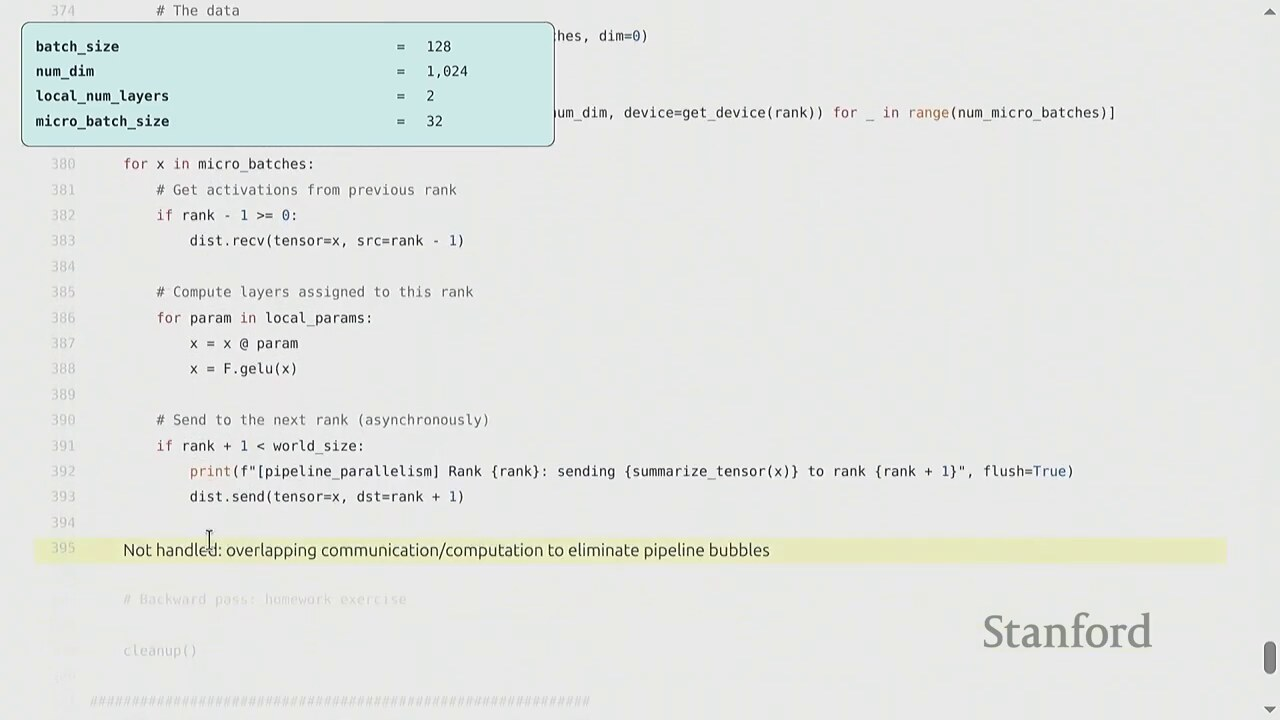
\includegraphics[width=\textwidth]{figures/fig_21_pipeline_bubbles.jpg}
\caption{流水线气泡：朴素实现中 GPU 空闲的"气泡"区域\protect\footnotemark}
\end{figure}
\footnotetext{视频画面时间区间：00:49:45--00:50:15。}

朴素流水线并行有个致命问题：\textbf{气泡}。当 rank 0 在处理一个 batch 时，rank 1 只能\textbf{干等}，直到 rank 0 把结果传过来。这段时间 rank 1 完全空闲，这就是"气泡"——流水线越深、气泡占比越大，硬件利用率越低。

\begin{importantbox}{microbatch：缓解气泡的标准手段}
把一个 batch 切成 $M$ 个 \textbf{microbatch}，让它们像流水线上的工件一样\textbf{依次}进入流水线。当 microbatch 1 流到 rank 1 时，microbatch 2 正好可以在 rank 0 上开始算——于是大部分时间所有 rank 都在干活，气泡被压缩。

设 $N$ 为 stage 数（= world size），$M$ 为 microbatch 数，则气泡占比约为：

\[
\text{bubble fraction} = \frac{N - 1}{M + N - 1}
\]

\begin{itemize}
\item $M \gg N$ 时，气泡占比 $\to 0$（流水线被打满）。
\item $M = 1$ 时退化为朴素流水线，气泡最大。
\end{itemize}
\end{importantbox}

\subsection{send / recv：点对点通信}

\begin{figure}[H]
\centering
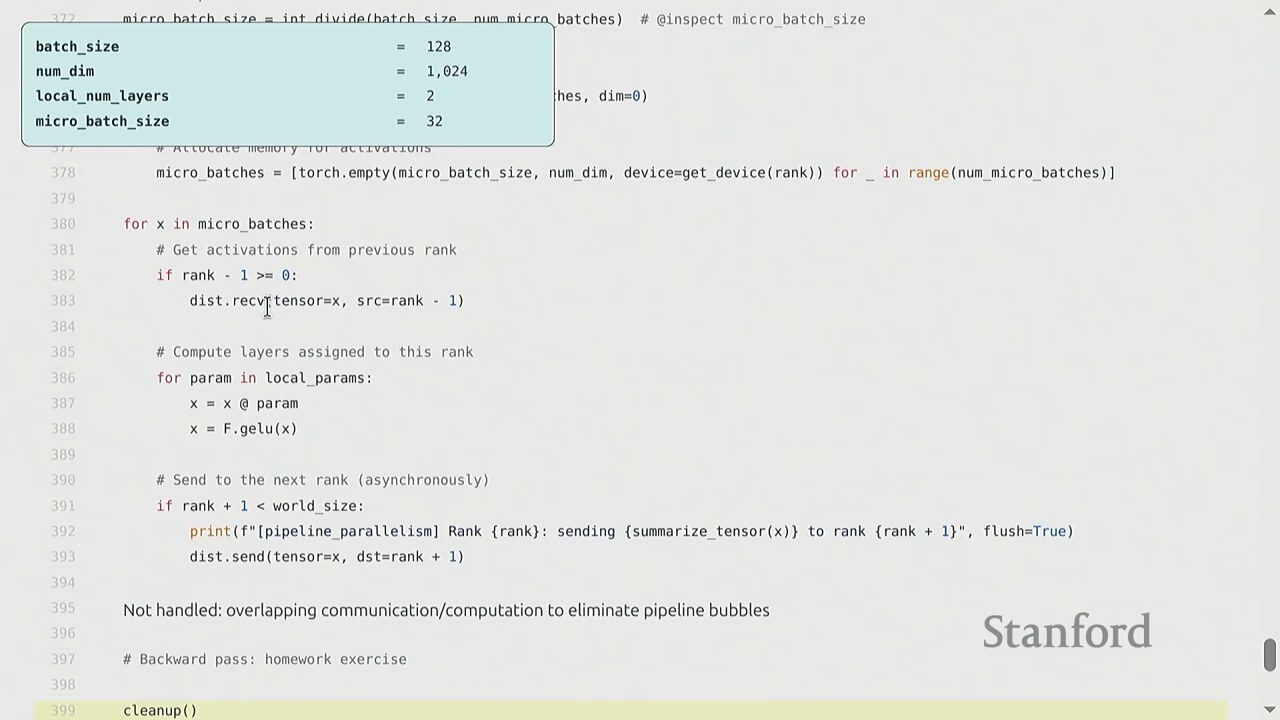
\includegraphics[width=\textwidth]{figures/fig_22_pipeline_send_recv.jpg}
\caption{流水线 send/recv：相邻 stage 用点对点原语传递激活\protect\footnotemark}
\end{figure}
\footnotetext{视频画面时间区间：00:52:15--00:52:45。}

与数据/张量并行用\textbf{集合}通信不同，流水线并行用\textbf{点对点}原语 \texttt{send / recv}：每个 rank 只和它的前驱/后继通信。

\begin{lstlisting}[language=Python]
for mb in microbatches:
    if rank > 0:
        x = recv(src=rank-1)        # 收前驱的激活
    x = forward(x, my_layers)        # 只算分给自己的层
    if rank < world_size - 1:
        send(x, dst=rank+1)          # 发给后继
\end{lstlisting}

\begin{warningbox}{最后一站与反向}
最后一个 rank（$N{-}1$）拿到完整的 forward 结果并计算 loss。\textbf{反向传播}则沿流水线逆向：从最后一个 rank 开始算梯度，用 \texttt{send/recv} 把梯度回传给前驱。朴素实现甚至没做反向（课上略过），但完整的流水线并行必须正确交错 forward 与 backward 的调度（如 1F1B、GPipe 等策略）。
\end{warningbox}

\subsection{通信与计算的重叠}

\begin{figure}[H]
\centering
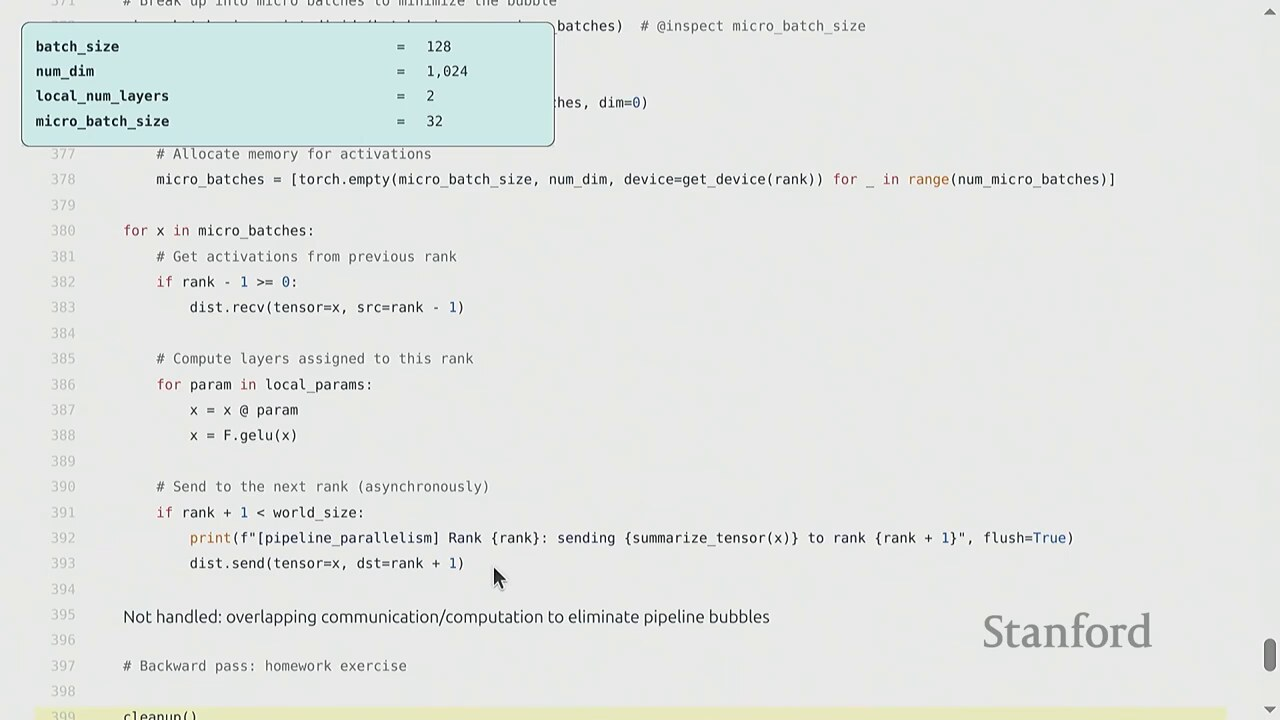
\includegraphics[width=\textwidth]{figures/fig_23_pipeline_overlap.jpg}
\caption{流水线通信-计算重叠：用异步 send/recv 隐藏通信延迟\protect\footnotemark}
\end{figure}
\footnotetext{视频画面时间区间：00:55:15--00:55:45。}

朴素实现里 \texttt{send/recv} 是\textbf{同步}的——发送方会阻塞直到接收方收完。理想做法是把它们改成\textbf{异步}：发送一个 microbatch 的同时，下一层已经开始计算上一个 microbatch。

\begin{knowledgebox}{同步范式 vs 异步范式}
现代大规模训练\textbf{几乎全是同步范式}——所有 rank 在 lock step 下工作，梯度严格对齐。10 多年前曾流行过\textbf{异步训练}（asynchronous）：用一个 parameter server，worker 随时上传梯度、随时拉参数，worker 挂了也能容错。但异步会引入\textbf{梯度陈旧}（staleness），在超大规模下反而更难收敛，所以工业界最终回归同步。Percy 特别澄清：他说的"workers 异步运行"只是指它们是\textbf{不同进程}，但执行逻辑上仍是严格同步的。
\end{knowledgebox}

\section{3D 并行、FSDP 与声明式分片}
\label{sec:3d}

\subsection{三种并行的组合：3D Parallelism}

\begin{figure}[H]
\centering
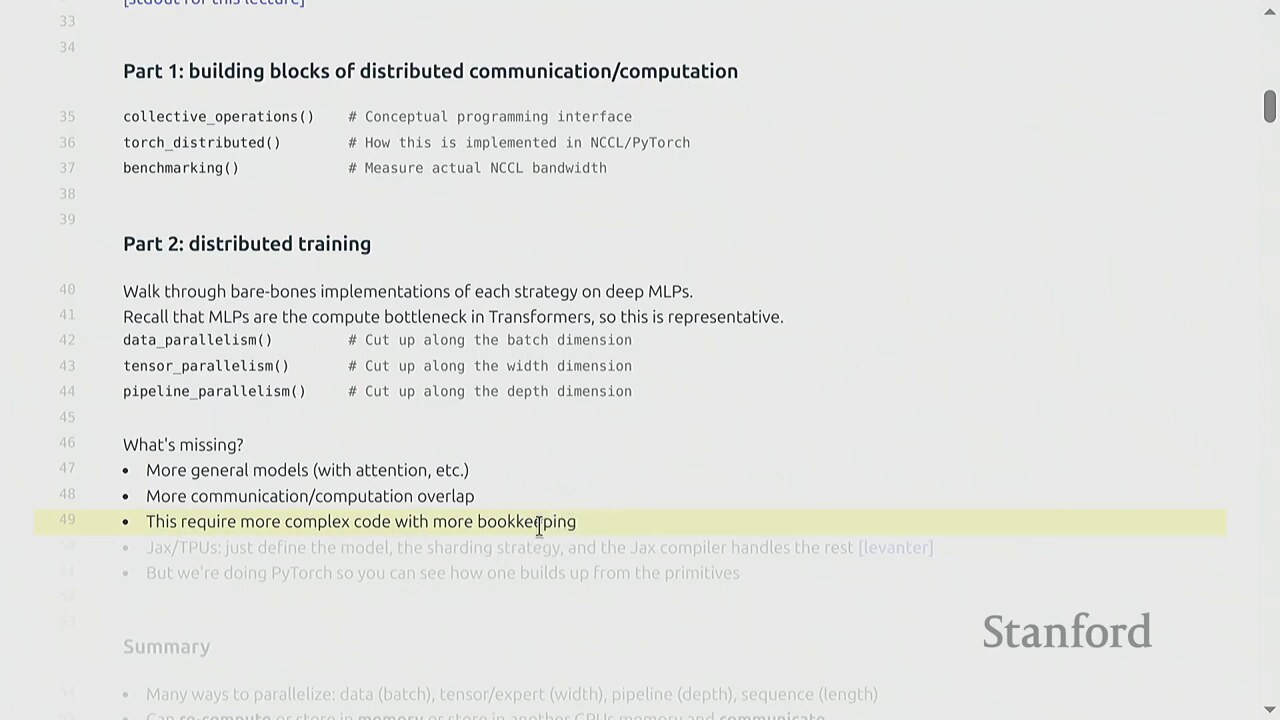
\includegraphics[width=\textwidth]{figures/fig_24_3d_parallelism.jpg}
\caption{3D 并行：DP + TP + PP 三种方式各用不同维度，组合使用\protect\footnotemark}
\end{figure}
\footnotetext{视频画面时间区间：00:57:45--00:58:15。}

真实的大模型训练从不是单一并行，而是\textbf{三者组合}。每个维度对应一个"轴"，集群被组织成 3D 网格：

\begin{tabular}{p{2cm}p{4cm}p{8cm}}
\toprule
\textbf{并行} & \textbf{切分对象} & \textbf{典型部署位置} \\
\midrule
TP & 模型宽度 & \textbf{节点内}（NVLink，带宽极高，否则太慢） \\
PP & 模型深度 & 节点间或节点内（中等带宽即可，通信少） \\
DP & 数据 & 节点间（all-reduce 可靠以太网承载） \\
\bottomrule
\end{tabular}

\begin{importantbox}{3D 并行的直觉}
把集群分成若干组：组内做 TP（紧密耦合、高带宽），若干 TP 组串成 PP 流水线，再在多条流水线间做 DP（松耦合、all-reduce）。例如训一个超大模型，可能用 8 卡 TP（一个节点） $\times$ 4 stage PP $\times$ 64 路 DP = 2048 卡。
\end{importantbox}

\subsection{FSDP 与 ZeRO：参数分片}

\begin{figure}[H]
\centering
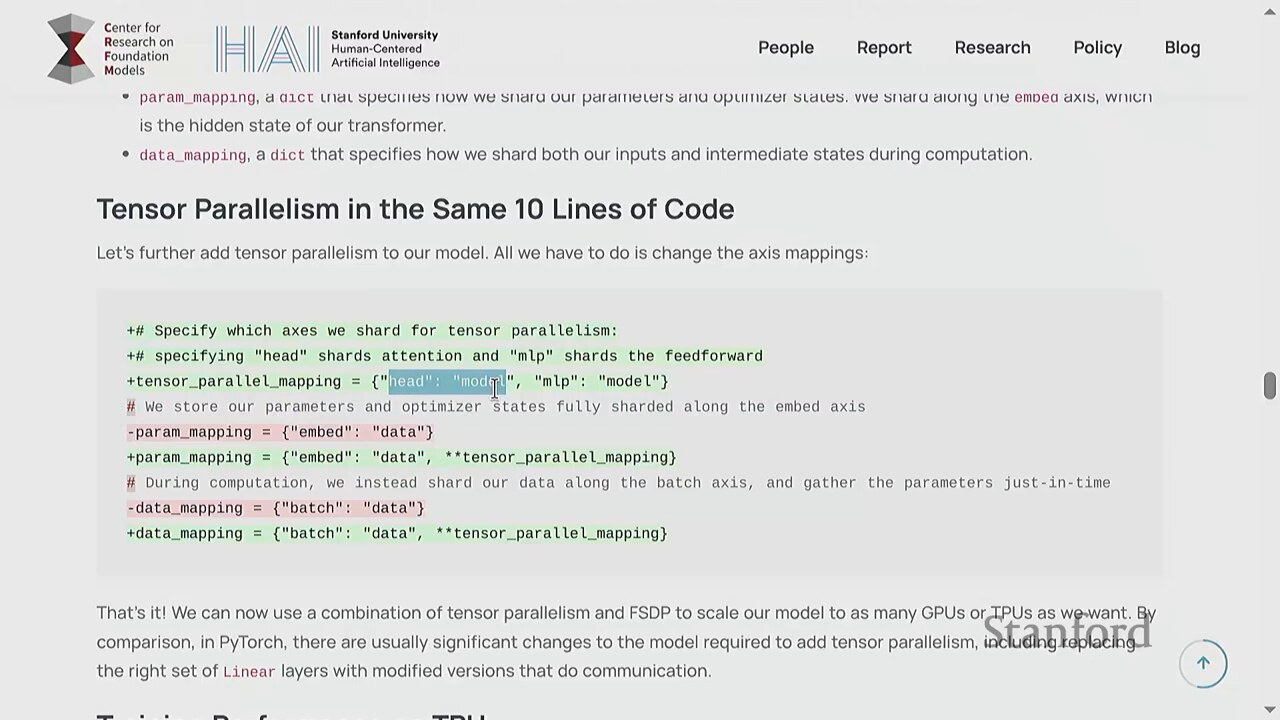
\includegraphics[width=\textwidth]{figures/fig_25_fdsp_zero.jpg}
\caption{FSDP / 参数分片（sharding）：声明式定义分片策略，按需 all-gather 还原参数\protect\footnotemark}
\end{figure}
\footnotetext{视频画面时间区间：00:59:45。}

\textbf{FSDP（Fully Sharded Data Parallel）}是数据并行的进化版：DP 要求每卡存\textbf{完整}参数，而 FSDP 把参数、梯度、优化器状态都\textbf{分片}到各卡，只在需要时按需 \textbf{all-gather} 还原。这直接对应 \textbf{ZeRO} 的三个阶段：

\begin{tabular}{p{2cm}p{4cm}p{8cm}}
\toprule
\textbf{ZeRO 阶段} & \textbf{分片对象} & \textbf{显存节省} \\
\midrule
ZeRO-1 & 优化器状态 & $\sim$4x（相对纯 DP） \\
ZeRO-2 & $+$ 梯度 & $\sim$8x \\
ZeRO-3 & $+$ 参数（= FSDP） & $\sim$N 倍（N 为 GPU 数） \\
\bottomrule
\end{tabular}

\begin{knowledgebox}{ZeRO-3 / FSDP 的核心机制}
前向/反向到某一层时，先 \textbf{all-gather} 把该层完整参数临时拉到本卡，算完立即\textbf{丢弃}（释放显存），只保留自己的那一片分片。这样任意时刻每卡只持有一层的完整副本 + 所有层的 $\frac{1}{N}$ 分片。代价是\textbf{通信量增加}（每层都要 all-gather），但换来的是：\textbf{能用更多卡训更大模型}。这正是"用额外通信换显存"的经典 trade-off。
\end{knowledgebox}

\subsection{PyTorch 手动实现 vs Jax 声明式分片}

Percy 指出，本讲手写的 MLP 版本是为了让你\textbf{看清底层}（哪些 all-gather、哪些 send/recv），但真实工程中\textbf{没人从零写这些}。两条路线：

\begin{itemize}
\item \textbf{PyTorch 手动路线}：Megatron-LM、PyTorch FSDP。代码"相当 hairy"，因为要处理任意架构的参数 bookkeeping——哪些层怎么切、shape 怎么对齐、梯度怎么同步。
\item \textbf{Jax 声明式路线}：只需\textbf{声明}分片策略（哪个维度切、映射到哪些 TPU），编译器自动生成集合通信代码。Stanford 开发的 \textbf{Lavanter}（基于 Jax）让 FSDP/TP 在 10 行内搞定。
\end{itemize}

\begin{practicebox}{课程为何坚持 PyTorch}
Jax 的声明式分片概念上更简洁，但 CS336 坚持 PyTorch，因为\textbf{只有亲手写过 all-gather 和 reduce-scatter，你才能真正理解通信在发生什么}。Lavanter 这类工具是"魔法"，而本课程的目标正是拆穿魔法。理解了底层，再用高层工具时你才知道边界在哪。
\end{practicebox}

\section{总结与延伸}

\subsection{核心论点}

\begin{importantbox}{五个核心论点}
\begin{enumerate}
\item \textbf{并行的本质是切维度}：DP 切 batch、TP 切宽度、PP 切深度。理解每种方式切哪个维度，其余都是推论。
\item \textbf{集合通信是字母表}：七个原语（broadcast/scatter/gather/reduce/all-reduce/reduce-scatter/all-gather）组合出所有并行策略。最关键的恒等式是 all-reduce = reduce-scatter + all-gather。
\item \textbf{通信成本可计算}：知道一次操作搬多少字节、硬件带宽多少，就能预测瓶颈。all-reduce 的 2x 因子、reduce-scatter 的无 2x，都来自字节计数。
\item \textbf{朴素实现有气泡}：流水线并行的气泡可用 microbatch 缓解；现代训练几乎全用同步范式。
\item \textbf{3D 并行 + FSDP 是工业现实}：TP 在节点内、PP 跨 stage、DP 跨副本；FSDP/ZeRO-3 用分片换显存，用通信换可扩展性。
\end{enumerate}
\end{importantbox}

\subsection{课堂问答：硬件演进与持续训练}

讲课后半段是开放的问答环节，几个问题切中了大规模训练的长期趋势，值得记录。

\begin{knowledgebox}{专用硬件会取代 GPU 吗？}
有听众问：GPU 会不会被 Transformer 专用的硬件取代？Percy 指出，在\textbf{推理}侧，专用硬件（如 Groq、Cerebras）已经相当活跃，它们的核心优势是\textbf{巨大的片上存储}——把尽可能多的权重和激活留在芯片内部，避免昂贵的显存搬运。Cerebras 甚至做到了一个"巨大的 L1 cache"，让你几乎不必把数据搬到片外。GPU 其实背着不少历史包袱（为图形渲染时代的分支计算、临时计算设计），这些在深度学习里并不需要，因此专用硬件有切实的改进空间。但在通用训练上，GPU 短期内仍是主流。
\end{knowledgebox}

\begin{importantbox}{这些技术能用于持续训练吗？}
有人问：本讲假设"从头一次性训练"，这些并行技术能否用于\textbf{增量/持续训练}（新数据来了不重训，而是增量补全）？Percy 的回答很干脆：\textbf{完全可以}。这些并行策略的工作单元就是"梯度步"，你只要从一个已有的 checkpoint 恢复，就能继续做梯度下降——没有任何东西要求你必须从零开始。持续训练在工程上与从头训练共享同一套并行基础设施，区别只在于数据流和学习率调度。
\end{importantbox}

\begin{warningbox}{Checkpoint 的位置选择}
另一个细节问题：流水线/张量并行中，激活该在\textbf{哪些位置}存 checkpoint（以省显存）？Percy 的经验法则是"每隔几层存一次"，尤其要选在那些\textbf{容易重新计算}的边界——比如 MLP 之后再接一个逐点线性层，这种"两步几乎等价于一步"的地方，没必要存两份激活，存一份即可。这正是"用额外计算换显存"思想在并行场景下的具体应用。
\end{warningbox}

\subsection{三种并行的对比总结}

\begin{tabular}{p{2cm}p{2.5cm}p{2.5cm}p{2.5cm}p{2.5cm}}
\toprule
\textbf{维度} & \textbf{DP} & \textbf{TP} & \textbf{PP} & \textbf{FSDP} \\
\midrule
切分对象 & 数据 & 模型宽度 & 模型深度 & 参数+梯度+优化器 \\
通信原语 & all-reduce & all-gather & send/recv & all-gather + reduce-scatter \\
通信频率 & 每步一次 & 每层一次 & 每 stage 一次 & 每层按需 \\
互连要求 & 中（以太网可） & \textbf{极高}（NVLink） & 中低 & 中高 \\
显存节省 & 无 & 中（参数分片） & 中（层分片） & \textbf{最大}（全分片） \\
\bottomrule
\end{tabular}

\subsection{下节预告与配套阅读}

接下来将进入 systems 模块的更深层，或转向 scaling laws / data 等模块。以下是建议按进度阅读的配套论文：

\begin{tabular}{p{7cm}p{6cm}}
\toprule
\textbf{论文/资源} & \textbf{对应知识点} \\
\midrule
Megatron-LM (Shoeybi et al.) & 张量并行的列/行切分优化 \\
ZeRO: Optimizing 500B Training (Rajbhandari et al.) & ZeRO-1/2/3 与 FSDP \\
PyTorch FSDP 文档 & 参数分片、按需 all-gather \\
GPipe / PipeDream & 流水线并行调度、气泡分析 \\
NCCL 文档 & ring all-reduce 的底层实现 \\
Lavanter (Jax) & 声明式分片的对比视角 \\
\bottomrule
\end{tabular}

%% --- 正文内容结束 ---

\end{document}
